\documentclass[12pt]{beamer}\usepackage[]{graphicx}\usepackage[]{color}
%% maxwidth is the original width if it is less than linewidth
%% otherwise use linewidth (to make sure the graphics do not exceed the margin)
\makeatletter
\def\maxwidth{ %
  \ifdim\Gin@nat@width>\linewidth
    \linewidth
  \else
    \Gin@nat@width
  \fi
}
\makeatother

\definecolor{fgcolor}{rgb}{0.345, 0.345, 0.345}
\newcommand{\hlnum}[1]{\textcolor[rgb]{0.686,0.059,0.569}{#1}}%
\newcommand{\hlstr}[1]{\textcolor[rgb]{0.192,0.494,0.8}{#1}}%
\newcommand{\hlcom}[1]{\textcolor[rgb]{0.678,0.584,0.686}{\textit{#1}}}%
\newcommand{\hlopt}[1]{\textcolor[rgb]{0,0,0}{#1}}%
\newcommand{\hlstd}[1]{\textcolor[rgb]{0.345,0.345,0.345}{#1}}%
\newcommand{\hlkwa}[1]{\textcolor[rgb]{0.161,0.373,0.58}{\textbf{#1}}}%
\newcommand{\hlkwb}[1]{\textcolor[rgb]{0.69,0.353,0.396}{#1}}%
\newcommand{\hlkwc}[1]{\textcolor[rgb]{0.333,0.667,0.333}{#1}}%
\newcommand{\hlkwd}[1]{\textcolor[rgb]{0.737,0.353,0.396}{\textbf{#1}}}%
\let\hlipl\hlkwb

\usepackage{framed}
\makeatletter
\newenvironment{kframe}{%
 \def\at@end@of@kframe{}%
 \ifinner\ifhmode%
  \def\at@end@of@kframe{\end{minipage}}%
  \begin{minipage}{\columnwidth}%
 \fi\fi%
 \def\FrameCommand##1{\hskip\@totalleftmargin \hskip-\fboxsep
 \colorbox{shadecolor}{##1}\hskip-\fboxsep
     % There is no \\@totalrightmargin, so:
     \hskip-\linewidth \hskip-\@totalleftmargin \hskip\columnwidth}%
 \MakeFramed {\advance\hsize-\width
   \@totalleftmargin\z@ \linewidth\hsize
   \@setminipage}}%
 {\par\unskip\endMakeFramed%
 \at@end@of@kframe}
\makeatother

\definecolor{shadecolor}{rgb}{.97, .97, .97}
\definecolor{messagecolor}{rgb}{0, 0, 0}
\definecolor{warningcolor}{rgb}{1, 0, 1}
\definecolor{errorcolor}{rgb}{1, 0, 0}
\newenvironment{knitrout}{}{} % an empty environment to be redefined in TeX

\usepackage{alltt}
%\usepackage[dvipsnames]{}
\IfFileExists{upquote.sty}{\usepackage{upquote}}{}
\begin{document}




\title{\textsc{statistical methods in r} }
\subtitle{Lubor Homolka}
\date{September $11^{\text{th}}$, 2018}

\begin{frame}
\titlepage
\end{frame}

%-----------

\begin{frame}
 \tableofcontents
\end{frame}

%-----------

\begin{frame}[fragile]\footnotesize
\frametitle{}

\begin{knitrout}
\definecolor{shadecolor}{rgb}{0.969, 0.969, 0.969}\color{fgcolor}\begin{kframe}
\begin{alltt}
\hlkwd{str}\hlstd{(mtcars)}
\end{alltt}
\begin{verbatim}
## 'data.frame':	32 obs. of  11 variables:
##  $ mpg : num  21 21 22.8 21.4 18.7 18.1 14.3 24.4 22.8 19.2 ...
##  $ cyl : num  6 6 4 6 8 6 8 4 4 6 ...
##  $ disp: num  160 160 108 258 360 ...
##  $ hp  : num  110 110 93 110 175 105 245 62 95 123 ...
##  $ drat: num  3.9 3.9 3.85 3.08 3.15 2.76 3.21 3.69 3.92 3.92 ...
##  $ wt  : num  2.62 2.88 2.32 3.21 3.44 ...
##  $ qsec: num  16.5 17 18.6 19.4 17 ...
##  $ vs  : num  0 0 1 1 0 1 0 1 1 1 ...
##  $ am  : num  1 1 1 0 0 0 0 0 0 0 ...
##  $ gear: num  4 4 4 3 3 3 3 4 4 4 ...
##  $ carb: num  4 4 1 1 2 1 4 2 2 4 ...
\end{verbatim}
\begin{alltt}
\hlstd{mtcars}\hlopt{$}\hlstd{mpg}
\end{alltt}
\begin{verbatim}
##  [1] 21.0 21.0 22.8 21.4 18.7 18.1 14.3 24.4 22.8 19.2 17.8 16.4 17.3 15.2
## [15] 10.4 10.4 14.7 32.4 30.4 33.9 21.5 15.5 15.2 13.3 19.2 27.3 26.0 30.4
## [29] 15.8 19.7 15.0 21.4
\end{verbatim}
\end{kframe}
\end{knitrout}

\end{frame}

%-----------

\begin{frame}\Huge \centering

{\Large Qualitative \& Quantitative Research}\vspace{2cm}

What's the difference?  \\{\Large(Statistical view)}

\end{frame}

%-----------

\begin{frame}\large
\frametitle{What qualitative researcher see...}

\begin{figure}
 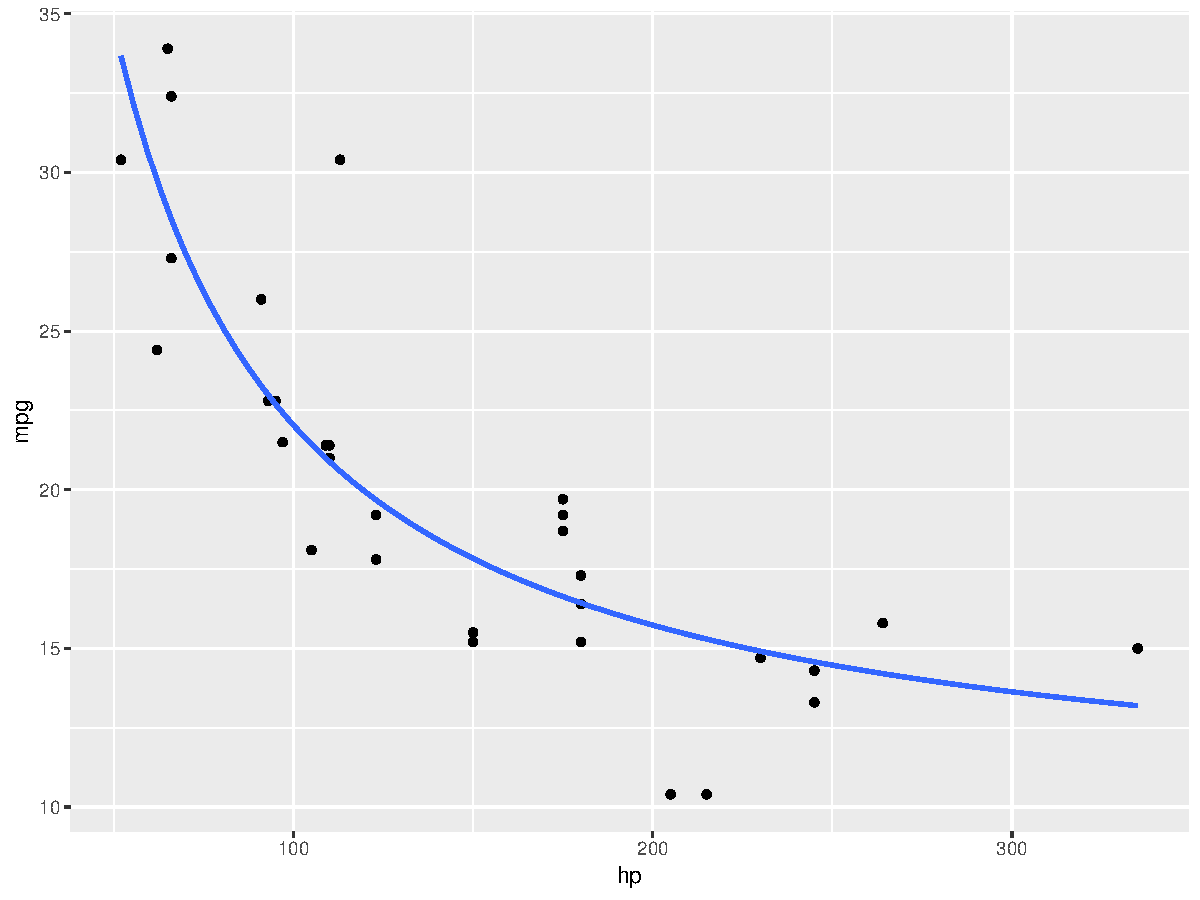
\includegraphics[width=0.7\paperwidth]{./Images/regQualit}
\end{figure}
\end{frame}


%-----------

\begin{frame}\large
\frametitle{What Quant See..}

\begin{figure}
 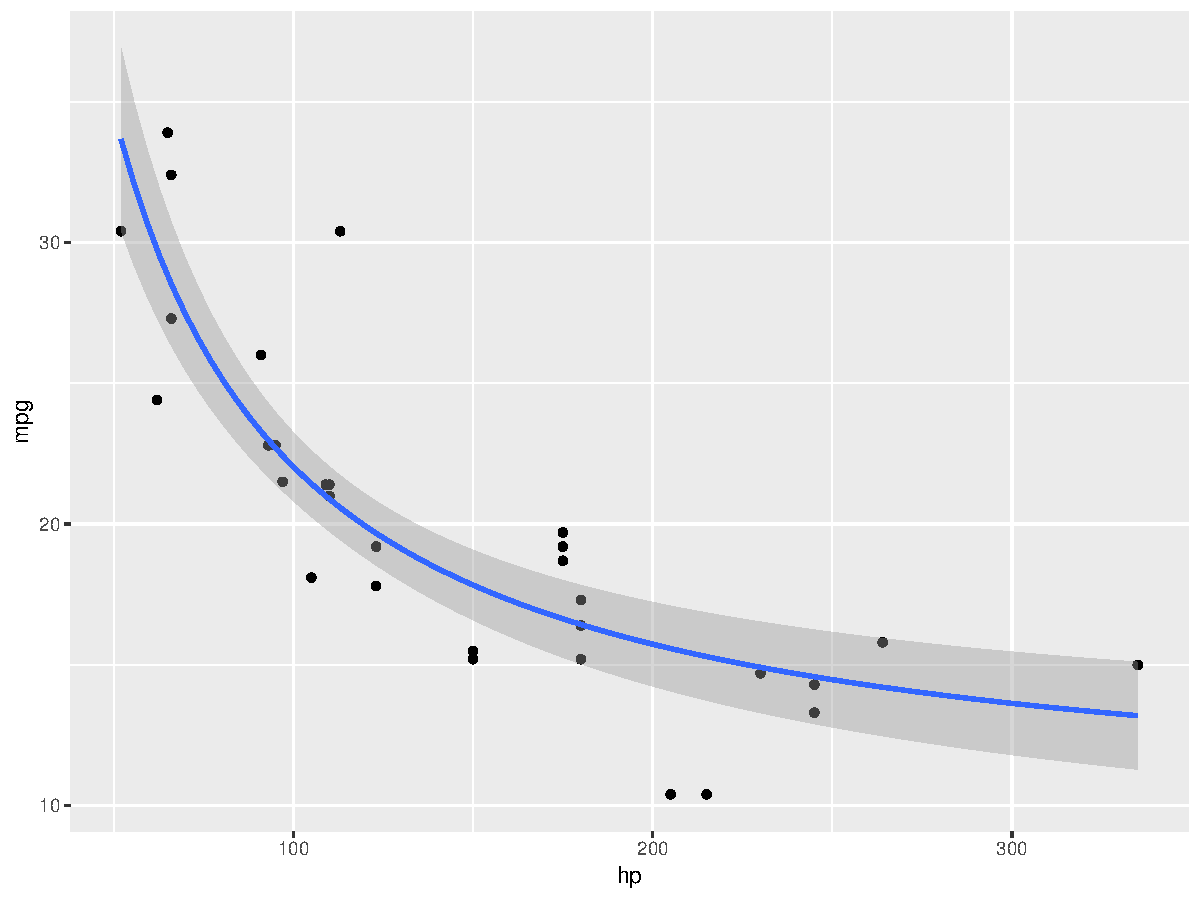
\includegraphics[width=0.7\paperwidth]{./Images/CIreg}
\end{figure}
\end{frame}

%-----------

\begin{frame}\large
\frametitle{If All Replications are observed}

\begin{figure}
 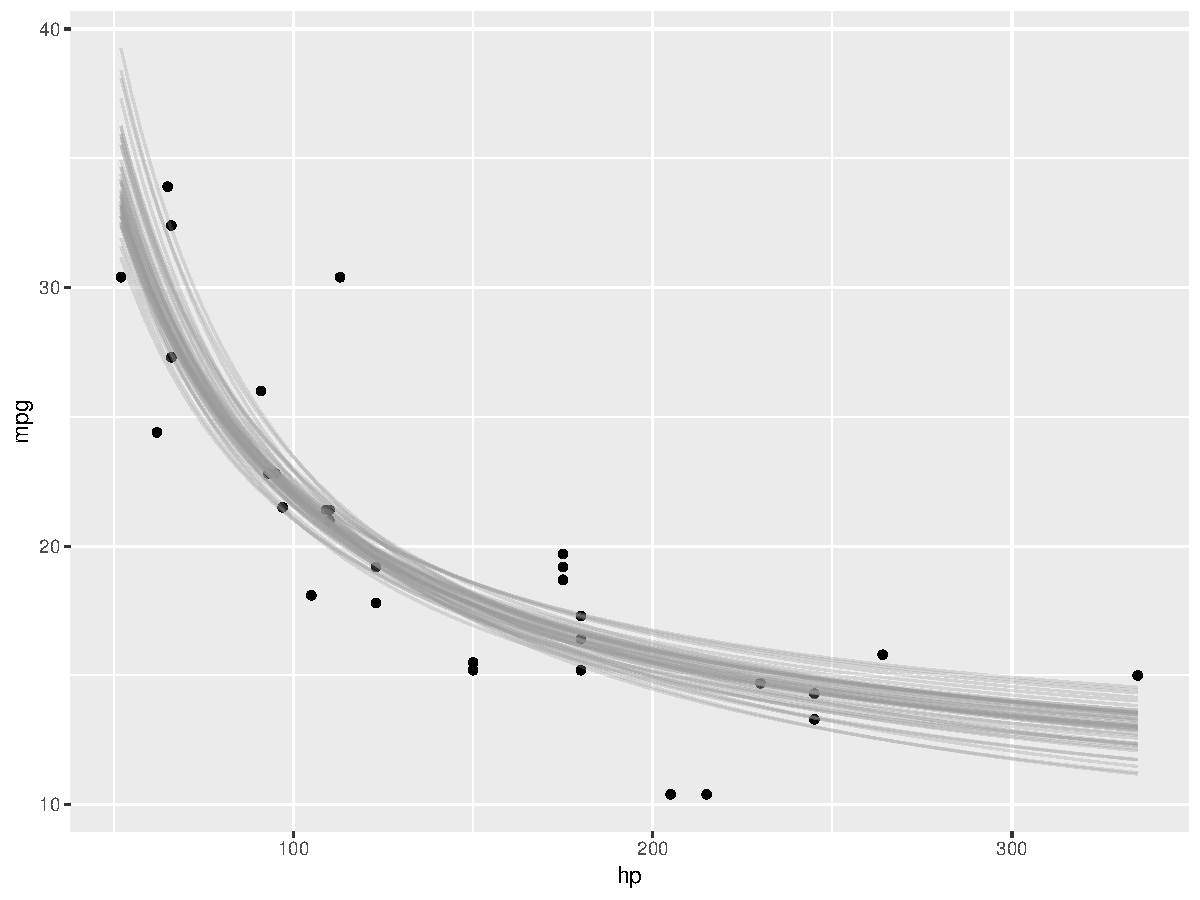
\includegraphics[width=0.7\paperwidth]{./Images/CIregLines}
\end{figure}
\end{frame}

%-----------

\begin{frame}\large
\frametitle{Do we need all the replications?}

\begin{figure}
 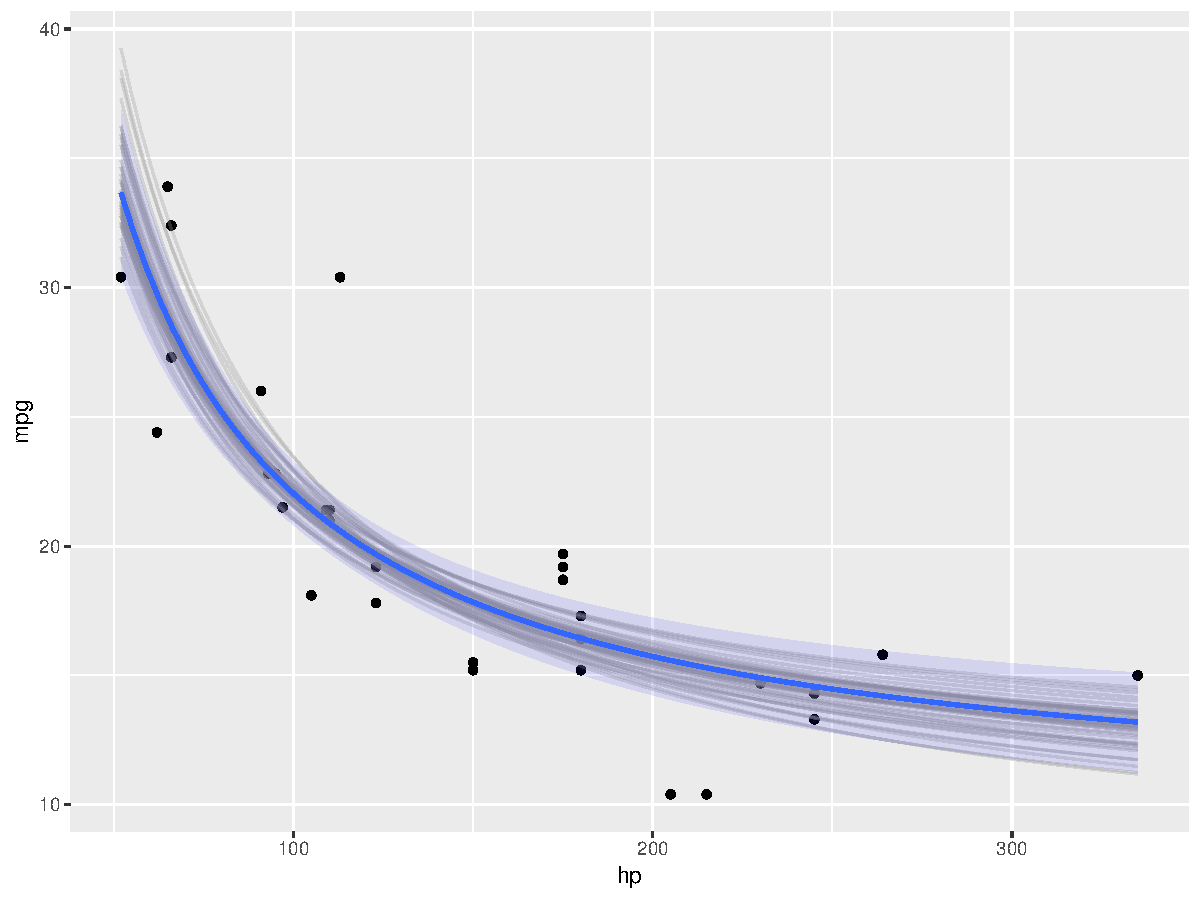
\includegraphics[width=0.7\paperwidth]{./Images/CItogether}
\end{figure}
\end{frame}

%-----------

\section{Standard Inferential Tests}

\begin{frame}\Large
\frametitle{What is Statistical Inference?}

\large{Statistical inferrence is a process of estimating a population characteristic based on the sample statistics.} \bigskip

\centering\begin{tabular}{c|c}
Sample &  Population \\ \hline 
$\bar{x}$ & $\mu$ \\ 
$r_{x_1x_2}$ & $\rho_{x_1x_2}$ \\ 
$y=b_0+b_1x$ & $y=\beta_0+\beta_1x$
\end{tabular} 

\end{frame}

%-----------

\begin{frame}\large
\frametitle{Tools of Statistical Inference}

\begin{itemize}
 \item Point estimate
 \item Interval estimate $\rightarrow$ confidence intervals
 \item Null hypothesis testing (NHST)
\end{itemize}

\onslide<2-> NHST: We try to falsify statement $H_0$ by finding a counter-proof stated in the $H_A$. 

\end{frame}

%-----------

    
    \begin{frame}[plain]
   \hspace*{-1.1cm} 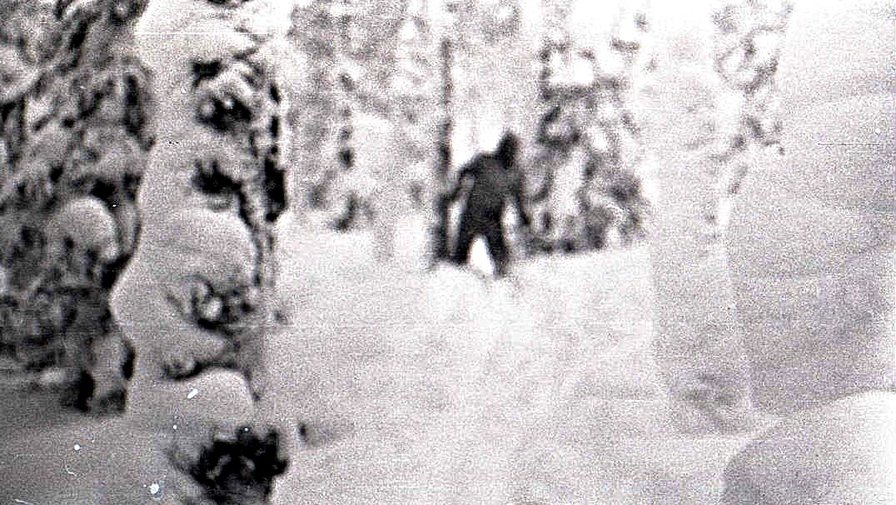
\includegraphics[height=\paperheight,width=\paperwidth]{./Images/yetti}
    \end{frame}
    

%-----------

\begin{frame}\large
\frametitle{Selected Test}

\begin{itemize}
 \item Test of Equal or Given Proportions
 \item Pearson's $\chi^2$ Test for Count Data
 \item Pearson \& Spearman correlation
 \item t-test
\end{itemize}

\end{frame}

%-----------

\begin{frame}\large
\frametitle{Test of Equal or Given Proportions}

This test tests whether the characteristics of the population \textcolor{blue}{$\pi$} can take some values.\bigskip

\textbf{Example:} You want to prove that the proportion of companies which are ready to adopt a new technology is smaller than \textcolor{blue}{50\%}. \smallskip\onslide<2->


\textcolor{red}{$H_0: \pi=0.5$ is what you want to disprove.} \smallskip

\textcolor{blue}{$H_A: \pi< 0.5$ is what you want to prove.}\bigskip\onslide<3->

You have asked 100 companies, 45 are ready.

\end{frame}

%-----------

\begin{frame}[fragile]

\frametitle{What do all these number mean?}

\begin{knitrout}\small
\definecolor{shadecolor}{rgb}{0.969, 0.969, 0.969}\color{fgcolor}\begin{kframe}
\begin{alltt}
\hlkwd{prop.test}\hlstd{(}\hlkwc{x}\hlstd{=}\hlnum{45}\hlstd{,} \hlkwc{n}\hlstd{=}\hlnum{100}\hlstd{,} \hlkwc{alternative}\hlstd{=}\hlstr{"less"}\hlstd{,} \hlkwc{p}\hlstd{=}\hlnum{0.5}\hlstd{)}
\end{alltt}
\begin{verbatim}
## 
## 	1-sample proportions test with continuity correction
## 
## data:  45 out of 100, null probability 0.5
## X-squared = 0.81, df = 1, p-value = 0.1841
## alternative hypothesis: true p is less than 0.5
## 95 percent confidence interval:
##  0.000000 0.537017
## sample estimates:
##    p 
## 0.45
\end{verbatim}
\end{kframe}
\end{knitrout}

\end{frame}

%-----------

\begin{frame}\large
\frametitle{Let's start with p-value}

\begin{equation}\nonumber
 \text{p-value} = P(\text{Data}\vert H_0=\text{TRUE})
\end{equation}

\onslide<2-> which is not 

\begin{equation}\nonumber
 P(H_0=\text{TRUE}\vert \text{Data})
\end{equation}

which is, what we want! \bigskip\onslide<3->

Data: possible results which would contradict $H_0$ and favour $H_A$ more than the observed result.

\end{frame}

%-----------

\begin{frame}[fragile]

\frametitle{Consider this Example with \textcolor{blue}{$H_A: \pi\neq 0.5$} }

\begin{knitrout}\small
\definecolor{shadecolor}{rgb}{0.969, 0.969, 0.969}\color{fgcolor}\begin{kframe}
\begin{alltt}
\hlkwd{prop.test}\hlstd{(}\hlkwc{x}\hlstd{=}\hlnum{45}\hlstd{,} \hlkwc{n}\hlstd{=}\hlnum{100}\hlstd{,} \hlkwc{alternative}\hlstd{=}\hlstr{"two.sided"}\hlstd{,} \hlkwc{p}\hlstd{=}\hlnum{0.5}\hlstd{)}
\end{alltt}
\begin{verbatim}
## 
## 	1-sample proportions test with continuity correction
## 
## data:  45 out of 100, null probability 0.5
## X-squared = 0.81, df = 1, p-value = 0.3681
## alternative hypothesis: true p is not equal to 0.5
## 95 percent confidence interval:
##  0.3514281 0.5524574
## sample estimates:
##    p 
## 0.45
\end{verbatim}
\end{kframe}
\end{knitrout}

Let's focus on Confidence intervals
\end{frame}

%-----------

\begin{frame}\large
\frametitle{Confidence Interval with $\alpha=0.9$}

\begin{figure}
\hspace*{-0.8cm} 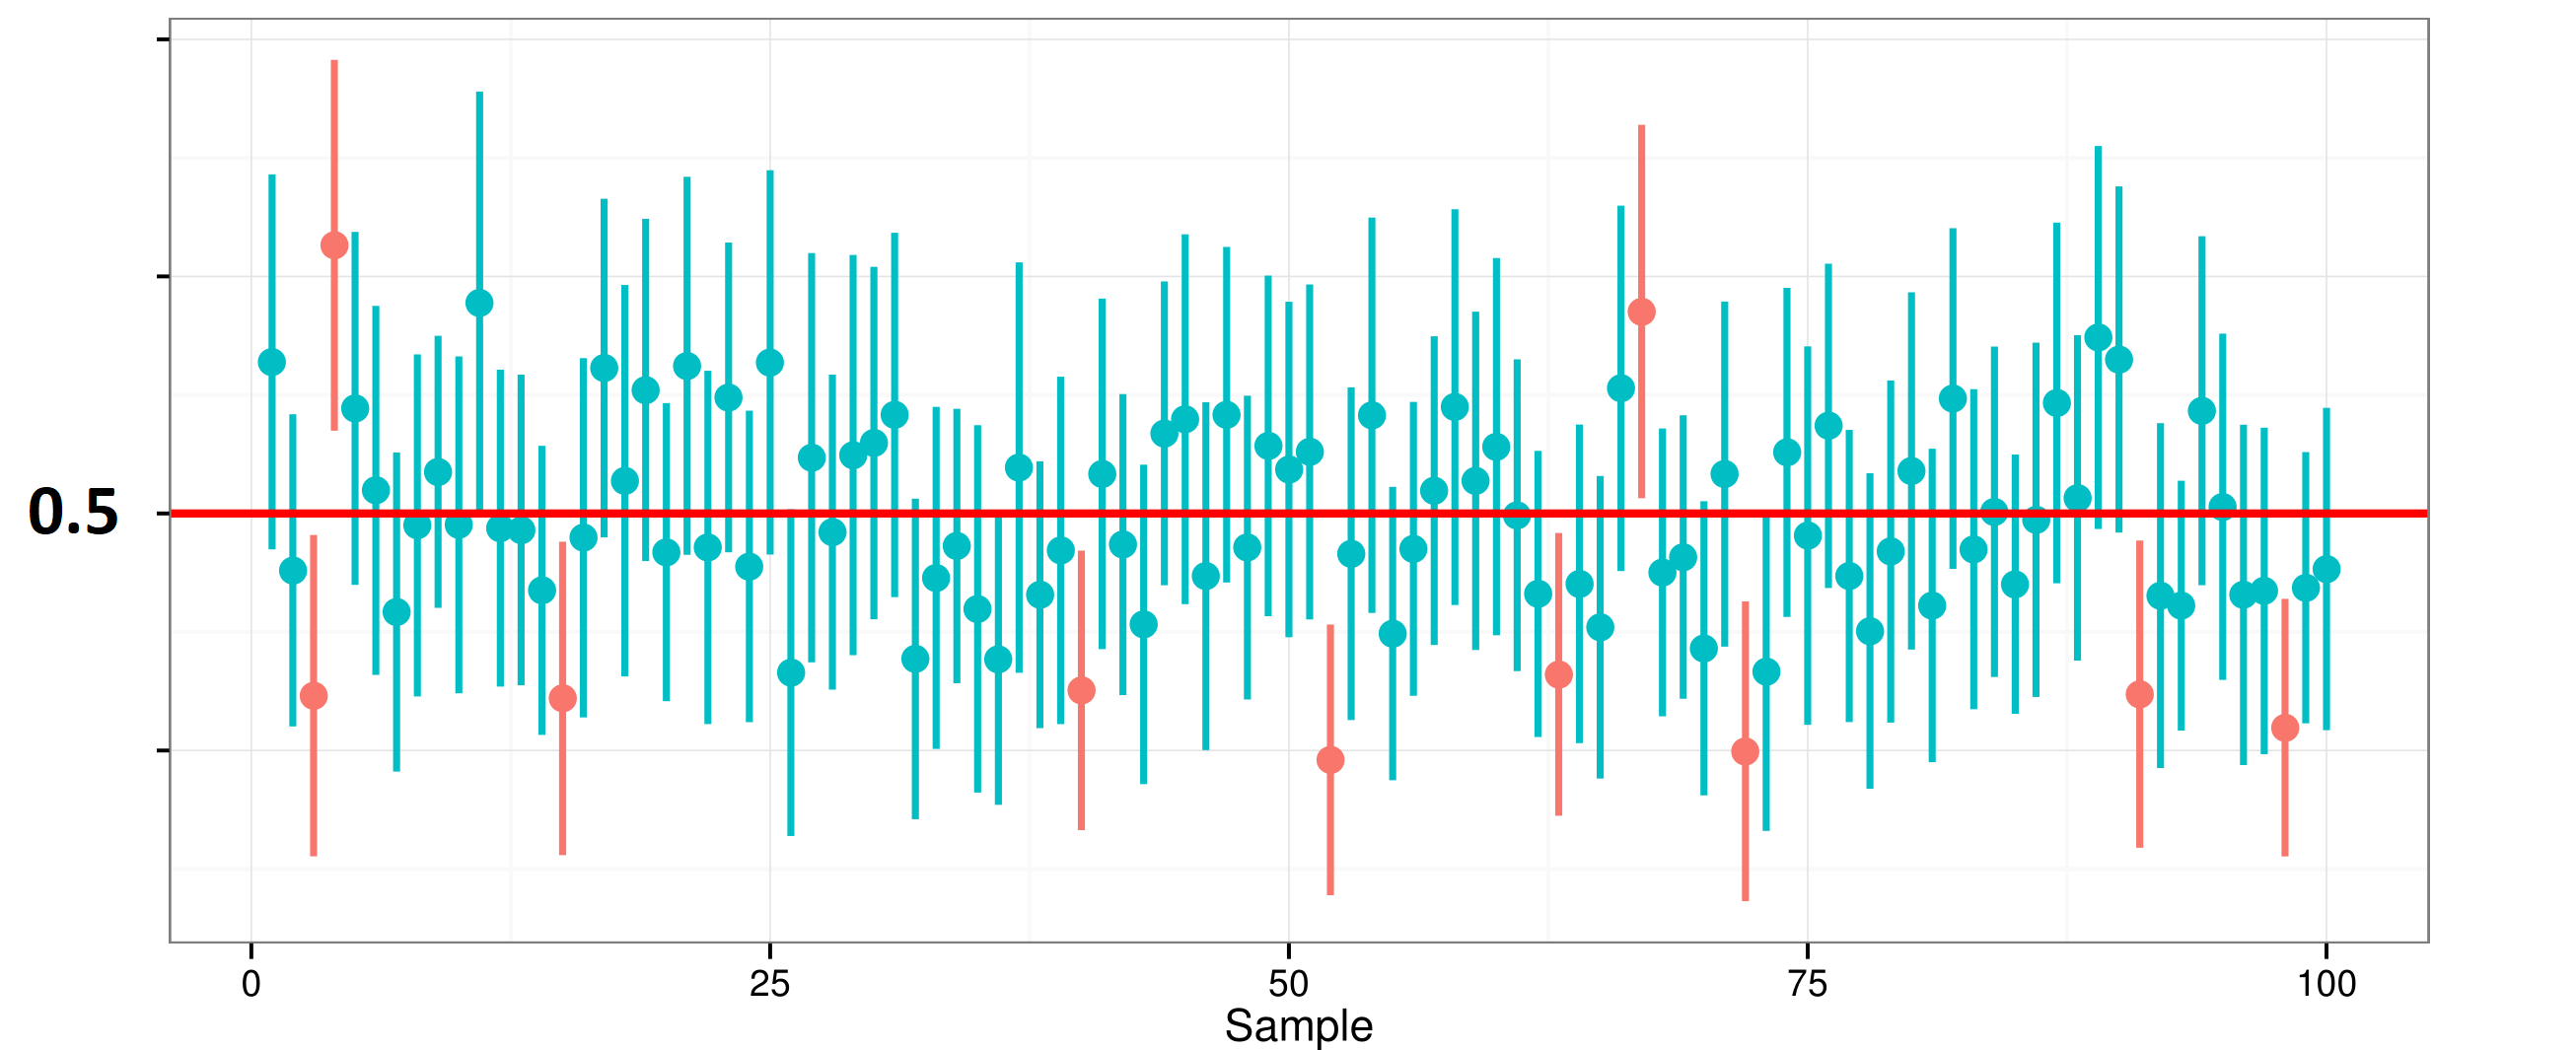
\includegraphics[width=1\paperwidth]{./Images/ci90.png}
\end{figure}
\end{frame}

%-----------

\begin{frame}\large
\frametitle{Confidence Interval with $\alpha=0.95$}

\begin{figure}
\hspace*{-0.8cm}  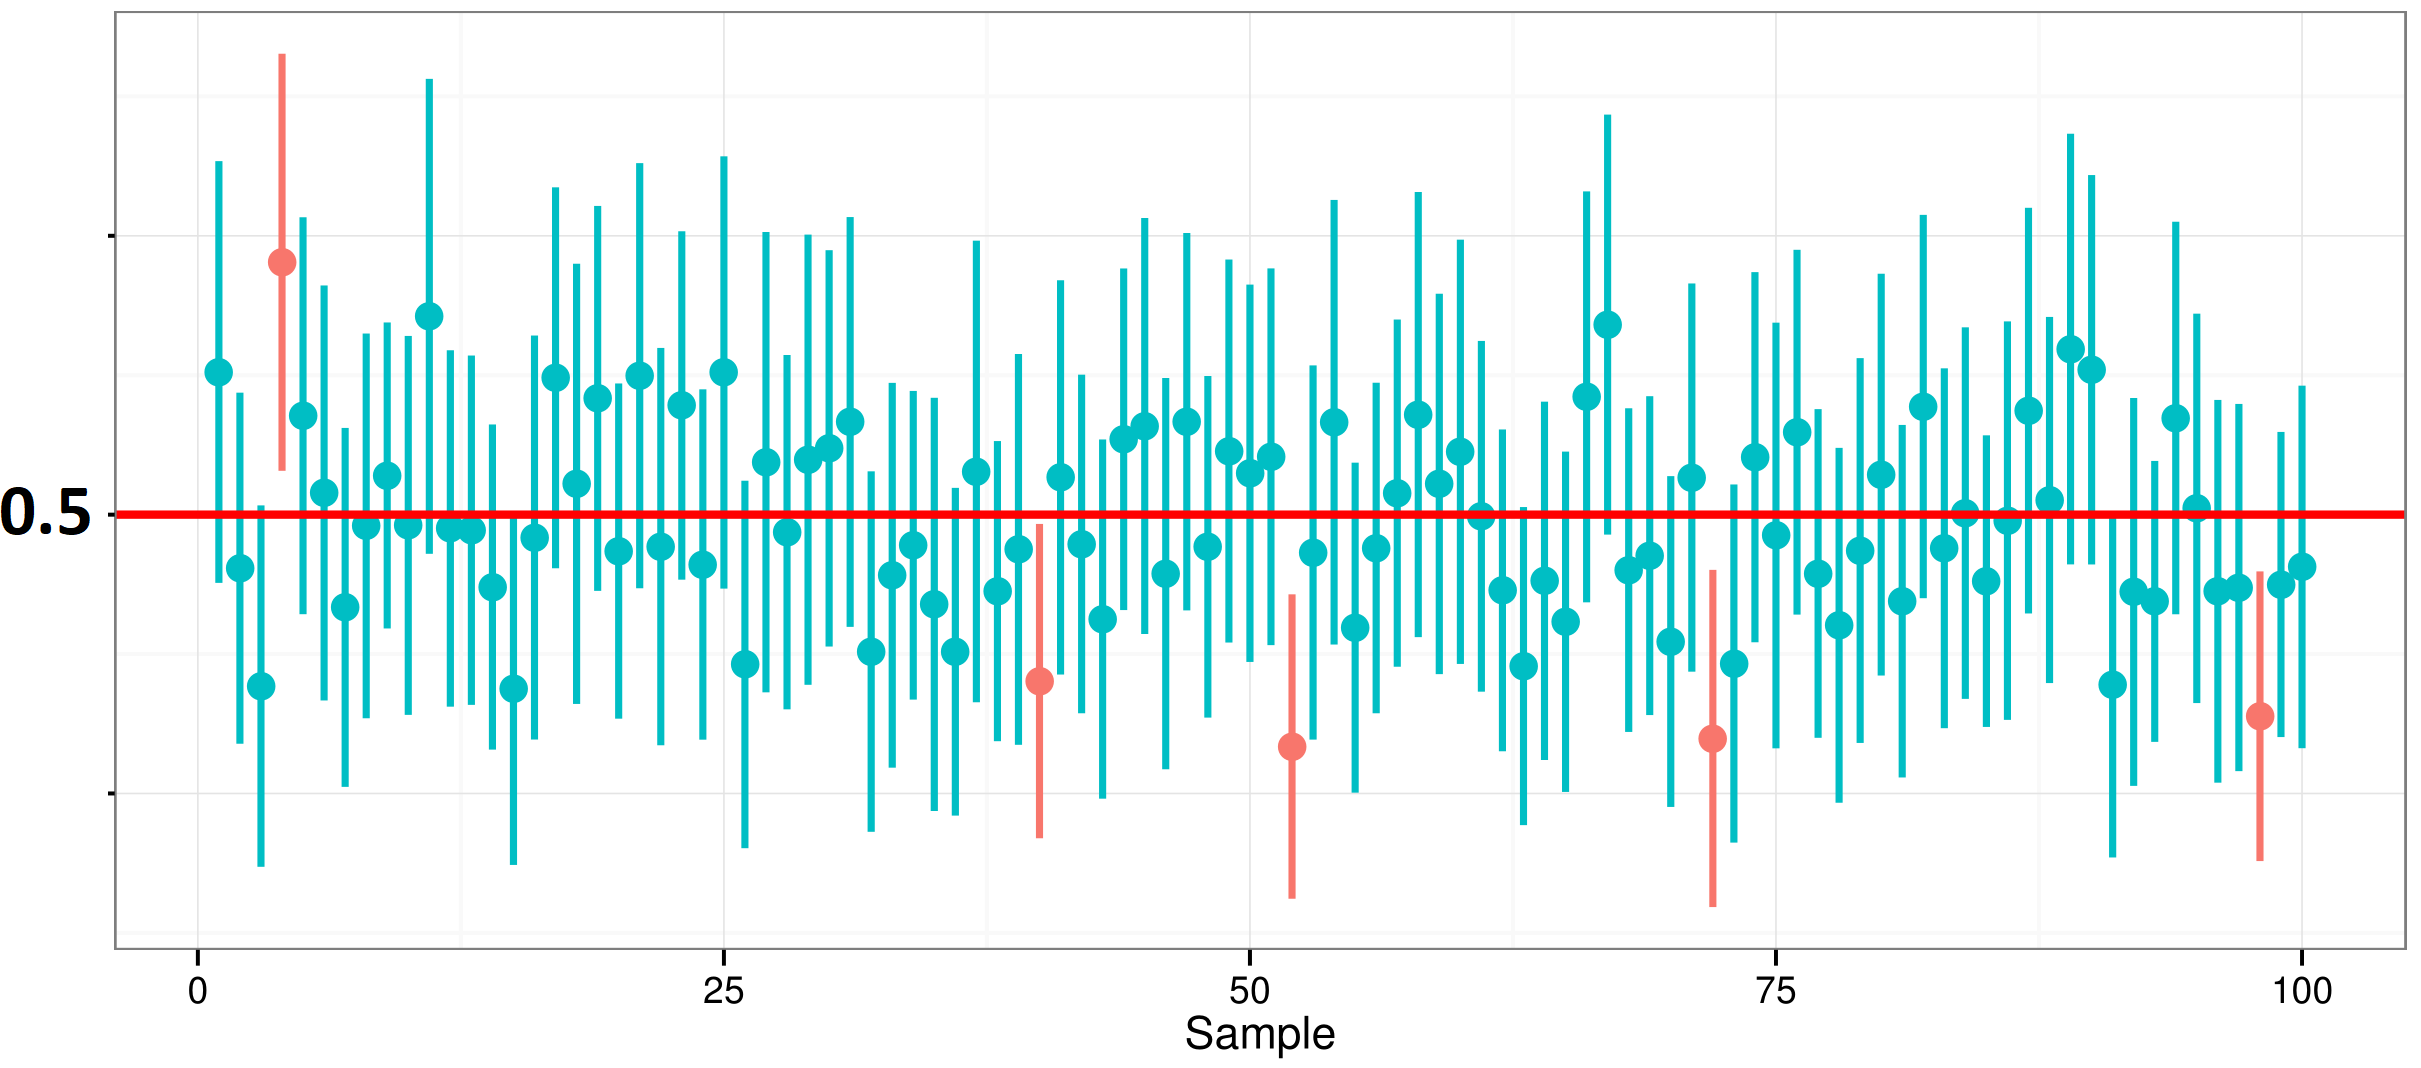
\includegraphics[width=0.95\paperwidth]{./Images/ci95.png}
\end{figure}
\end{frame}

%-----------

\begin{frame}[fragile]
\frametitle{Test of Equal or Given Proportions}

\begin{knitrout}\small
\definecolor{shadecolor}{rgb}{0.969, 0.969, 0.969}\color{fgcolor}\begin{kframe}
\begin{alltt}
\hlkwd{prop.test}\hlstd{(}\hlkwc{x}\hlstd{=}\hlnum{45}\hlstd{,} \hlkwc{n}\hlstd{=}\hlnum{100}\hlstd{,} \hlkwc{alternative}\hlstd{=}\hlstr{"less"}\hlstd{,} \hlkwc{p}\hlstd{=}\hlnum{0.5}\hlstd{)}
\end{alltt}
\begin{verbatim}
## 
## 	1-sample proportions test with continuity correction
## 
## data:  45 out of 100, null probability 0.5
## X-squared = 0.81, df = 1, p-value = 0.1841
## alternative hypothesis: true p is less than 0.5
## 95 percent confidence interval:
##  0.000000 0.537017
## sample estimates:
##    p 
## 0.45
\end{verbatim}
\end{kframe}
\end{knitrout}
\onslide<2-> Don't forget that no evidence for $\pi< 0.5$ does not imply evidence for $\pi=0.5$.
\end{frame}

%-----------

\begin{frame}[fragile]
\frametitle{Test of Equal or Given Proportions}

\begin{knitrout}\small
\definecolor{shadecolor}{rgb}{0.969, 0.969, 0.969}\color{fgcolor}\begin{kframe}
\begin{alltt}
\hlkwd{prop.test}\hlstd{(}\hlkwc{x}\hlstd{=}\hlnum{450}\hlstd{,} \hlkwc{n}\hlstd{=}\hlnum{1000}\hlstd{,} \hlkwc{alternative}\hlstd{=}\hlstr{"less"}\hlstd{,} \hlkwc{p}\hlstd{=}\hlnum{0.5}\hlstd{)}
\end{alltt}
\begin{verbatim}
## 
## 	1-sample proportions test with continuity correction
## 
## data:  450 out of 1000, null probability 0.5
## X-squared = 9.801, df = 1, p-value = 0.0008721
## alternative hypothesis: true p is less than 0.5
## 95 percent confidence interval:
##  0.0000000 0.4764786
## sample estimates:
##    p 
## 0.45
\end{verbatim}
\end{kframe}
\end{knitrout}

\end{frame}

%-----------

\begin{frame}[fragile]
\frametitle{Test of Equal or Given Proportions}

\begin{knitrout}\small
\definecolor{shadecolor}{rgb}{0.969, 0.969, 0.969}\color{fgcolor}\begin{kframe}
\begin{alltt}
\hlkwd{prop.test}\hlstd{(}\hlkwc{x}\hlstd{=}\hlnum{40}\hlstd{,} \hlkwc{n}\hlstd{=}\hlnum{100}\hlstd{,} \hlkwc{alternative}\hlstd{=}\hlstr{"less"}\hlstd{,} \hlkwc{p}\hlstd{=}\hlnum{0.5}\hlstd{)}
\end{alltt}
\begin{verbatim}
## 
## 	1-sample proportions test with continuity correction
## 
## data:  40 out of 100, null probability 0.5
## X-squared = 3.61, df = 1, p-value = 0.02872
## alternative hypothesis: true p is less than 0.5
## 95 percent confidence interval:
##  0.0000000 0.4872158
## sample estimates:
##   p 
## 0.4
\end{verbatim}
\end{kframe}
\end{knitrout}

\end{frame}

%-----------

\begin{frame}\large
\frametitle{Test of Equal or Given Proportions}

This test tests whether $k$ population \textcolor{blue}{$\pi$} differ .\bigskip

\textbf{Example:} You want to prove that the proportion of companies which are ready to adopt a new technology is smaller when the company is fully owned by Czech owners $\pi_1$, than proportion of international ready-companies $\pi_2$. \smallskip\onslide<2->


\textcolor{red}{$H_0: \pi_1=\pi_2$ is what you want to disprove.} \smallskip

\textcolor{blue}{$H_A: \pi_1< \pi_2$ is what you want to prove.}\bigskip\onslide<3->

You have asked 100 CZ and 100 Int companies. 30CZ and 40Int companies are ready.

\end{frame}

%-----------

\begin{frame}[fragile]
\frametitle{Test of Equal or Given Proportions}

\begin{knitrout}\small
\definecolor{shadecolor}{rgb}{0.969, 0.969, 0.969}\color{fgcolor}\begin{kframe}
\begin{alltt}
\hlkwd{prop.test}\hlstd{(}\hlkwc{x}\hlstd{=}\hlkwd{c}\hlstd{(}\hlnum{30}\hlstd{,} \hlnum{40}\hlstd{),} \hlkwc{n}\hlstd{=}\hlkwd{c}\hlstd{(}\hlnum{100}\hlstd{,} \hlnum{100}\hlstd{),} \hlkwc{alternative}\hlstd{=}\hlstr{"less"}\hlstd{)}
\end{alltt}
\begin{verbatim}
## 
## 	2-sample test for equality of proportions with continuity
## 	correction
## 
## data:  c(30, 40) out of c(100, 100)
## X-squared = 1.7802, df = 1, p-value = 0.09106
## alternative hypothesis: less
## 95 percent confidence interval:
##  -1.00000000  0.02034014
## sample estimates:
## prop 1 prop 2 
##    0.3    0.4
\end{verbatim}
\end{kframe}
\end{knitrout}

\end{frame}

%-----------

\begin{frame}\large
\frametitle{Pearson's $\chi^2$ Test for Count Data}

This test tests associatio between two non-numeric variables.\bigskip

\textbf{Example:} Example from Belas's Financial Markets book. Authors were intersted wheter Czech and Slovakian e-banking services are equally satisfied with the services. \smallskip\onslide<2->


\textcolor{red}{$H_0: \text{no assoc. between nationality and satisfaction}$} \smallskip

\textcolor{blue}{$H_A: \text{there is some assoc}$: this is what you want to prove.}\bigskip\onslide<3->

\end{frame}

%-----------

\begin{frame}[fragile]


\begin{knitrout}
\definecolor{shadecolor}{rgb}{0.969, 0.969, 0.969}\color{fgcolor}\begin{kframe}
\begin{alltt}
\hlkwd{head}\hlstd{(bankingData)}
\end{alltt}
\begin{verbatim}
##     country  satis
## 58       CZ    Yes
## 157      SK    Yes
## 81       CZ     No
## 174      SK     No
## 185      SK justOK
## 9        CZ    Yes
\end{verbatim}
\begin{alltt}
\hlstd{bankingData} \hlopt \hlstd{table}
\end{alltt}
\begin{verbatim}
##        satis
## country justOK No Yes
##      CZ     12 26  62
##      SK     16 23  61
\end{verbatim}
\end{kframe}
\end{knitrout}

\end{frame}

%-----------

\begin{frame}[fragile]

\begin{knitrout}
\definecolor{shadecolor}{rgb}{0.969, 0.969, 0.969}\color{fgcolor}\begin{kframe}
\begin{alltt}
\hlstd{tab} \hlkwb{<-} \hlstd{bankingData} \hlopt \hlstd{table} \hlopt \hlstd{t}
\hlkwd{chisq.test}\hlstd{(tab)}
\end{alltt}
\begin{verbatim}
## 
## 	Pearson's Chi-squared test
## 
## data:  tab
## X-squared = 0.76323, df = 2, p-value = 0.6828
\end{verbatim}
\end{kframe}
\end{knitrout}

Conclusion: There is no evidence for statistically significant associaton.
\end{frame}

%-----------

\begin{frame}[fragile]
Let's adjust the data to find association

\begin{knitrout}
\definecolor{shadecolor}{rgb}{0.969, 0.969, 0.969}\color{fgcolor}\begin{kframe}
\begin{alltt}
\hlstd{tab2} \hlkwb{<-} \hlkwd{matrix}\hlstd{(}\hlkwd{c}\hlstd{(}\hlnum{12}\hlstd{,}\hlnum{35}\hlstd{,}\hlnum{40}\hlstd{,}\hlnum{16}\hlstd{,}\hlnum{23}\hlstd{,}\hlnum{61}\hlstd{),} \hlkwc{ncol}\hlstd{=}\hlnum{3}\hlstd{,}
               \hlkwc{byrow} \hlstd{=} \hlnum{TRUE}\hlstd{)}
\hlstd{tab2}
\end{alltt}
\begin{verbatim}
##      [,1] [,2] [,3]
## [1,]   12   35   40
## [2,]   16   23   61
\end{verbatim}
\begin{alltt}
\hlkwd{prop.table}\hlstd{(tab2,} \hlnum{1}\hlstd{)} \hlcom{#1 means row margin}
\end{alltt}
\begin{verbatim}
##          [,1]      [,2]      [,3]
## [1,] 0.137931 0.4022989 0.4597701
## [2,] 0.160000 0.2300000 0.6100000
\end{verbatim}
\end{kframe}
\end{knitrout}

\end{frame}

%-----------

\begin{frame}[fragile]

\begin{knitrout}
\definecolor{shadecolor}{rgb}{0.969, 0.969, 0.969}\color{fgcolor}\begin{kframe}
\begin{alltt}
\hlkwd{chisq.test}\hlstd{(tab2)}
\end{alltt}
\begin{verbatim}
## 
## 	Pearson's Chi-squared test
## 
## data:  tab2
## X-squared = 6.5484, df = 2, p-value = 0.03785
\end{verbatim}
\end{kframe}
\end{knitrout}

Conclusion: We have an evidence for statistically significant associaton. \onslide<2-> What caused the association? We need to inspect results:
\end{frame}

%-----------

\begin{frame}[fragile]

\begin{knitrout}\small
\definecolor{shadecolor}{rgb}{0.969, 0.969, 0.969}\color{fgcolor}\begin{kframe}
\begin{alltt}
\hlstd{chTest} \hlkwb{<-} \hlkwd{chisq.test}\hlstd{(tab2)}
\hlkwd{str}\hlstd{(chTest)}
\end{alltt}
\begin{verbatim}
## List of 9
##  $ statistic: Named num 6.55
##   ..- attr(*, "names")= chr "X-squared"
##  $ parameter: Named int 2
##   ..- attr(*, "names")= chr "df"
##  $ p.value  : num 0.0378
##  $ method   : chr "Pearson's Chi-squared test"
##  $ data.name: chr "tab2"
##  $ observed : num [1:2, 1:3] 12 16 35 23 40 61
##  $ expected : num [1:2, 1:3] 13 15 27 31 47 ...
##  $ residuals: num [1:2, 1:3] -0.284 0.265 1.543 -1.439 -1.02 ...
##  $ stdres   : num [1:2, 1:3] -0.422 0.422 2.541 -2.541 -2.056 ...
##  - attr(*, "class")= chr "htest"
\end{verbatim}
\end{kframe}
\end{knitrout}

Residuals is the key factor. It tells us what goes against our expectation stated in the $H_0$. 

\end{frame}

%-----------

\begin{frame}[fragile]
\frametitle{}

\begin{knitrout}
\definecolor{shadecolor}{rgb}{0.969, 0.969, 0.969}\color{fgcolor}\begin{kframe}
\begin{alltt}
\hlstd{chTest}\hlopt{$}\hlstd{residuals}
\end{alltt}
\begin{verbatim}
##            [,1]      [,2]       [,3]
## [1,] -0.2844735  1.543147 -1.0196109
## [2,]  0.2653392 -1.439351  0.9510297
\end{verbatim}
\begin{alltt}
\hlstd{residChi} \hlkwb{<-} \hlstd{chTest}\hlopt{$}\hlstd{residuals} \hlopt \hlkwd{data.frame}\hlstd{()}
\hlkwd{colnames}\hlstd{(residChi)} \hlkwb{<-} \hlkwd{c}\hlstd{(}\hlstr{"justOK"}\hlstd{,} \hlstr{"No"}\hlstd{,} \hlstr{"Yes"}\hlstd{)}
\hlkwd{rownames}\hlstd{(residChi)} \hlkwb{<-} \hlkwd{c}\hlstd{(}\hlstr{"CZ"}\hlstd{,} \hlstr{"SK"}\hlstd{)}
\hlstd{residChi}
\end{alltt}
\begin{verbatim}
##        justOK        No        Yes
## CZ -0.2844735  1.543147 -1.0196109
## SK  0.2653392 -1.439351  0.9510297
\end{verbatim}
\end{kframe}
\end{knitrout}

\end{frame}

%-----------

\begin{frame}\large
\frametitle{Correlation Tests}

Test whether there is a relationship between two independent variables.\bigskip

\textbf{Example:} You have measured IQ of 50 respondents and their reaction time in seconds. You don't expect direct relations between variables. But you expect there is some degree of correlation. \smallskip\onslide<2->

\textcolor{red}{$H_0: \rho=0$ no correlation between variables} \smallskip

\textcolor{blue}{$H_A: \rho\neq 0$} 

\end{frame}

%-----------

\begin{frame}[fragile]



\begin{knitrout}\footnotesize
\definecolor{shadecolor}{rgb}{0.969, 0.969, 0.969}\color{fgcolor}\begin{kframe}
\begin{alltt}
\hlkwd{head}\hlstd{(dataCor,} \hlnum{3}\hlstd{)}
\end{alltt}
\begin{verbatim}
##   IQ  reaction
## 1 90  7.800140
## 2 90 10.324620
## 3 90  9.640206
\end{verbatim}
\begin{alltt}
\hlkwd{ggplot}\hlstd{(dataCor,} \hlkwd{aes}\hlstd{(}\hlkwc{x}\hlstd{=IQ,} \hlkwc{y}\hlstd{=reaction))} \hlopt{+} \hlkwd{geom_point}\hlstd{()}
\end{alltt}
\end{kframe}

{\centering 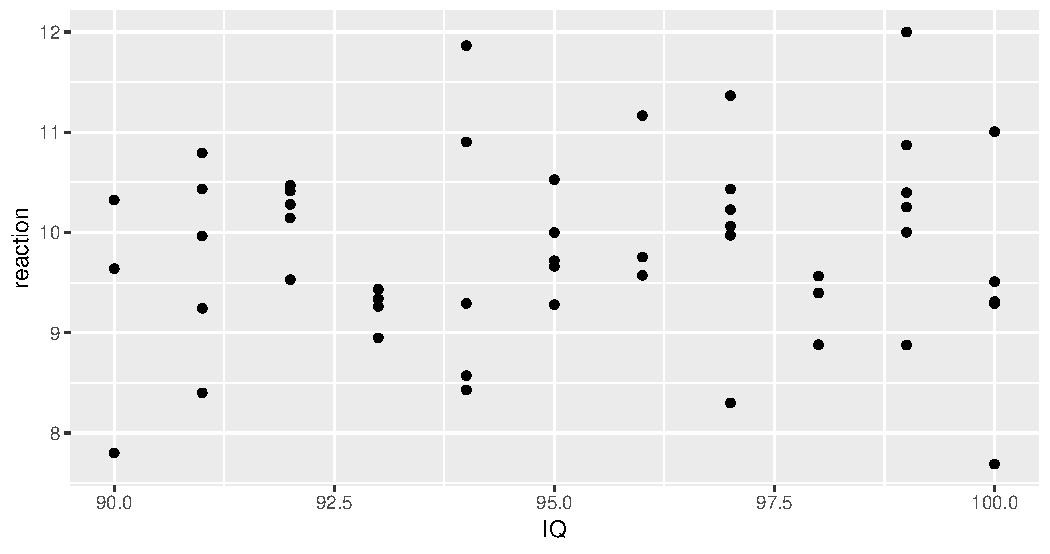
\includegraphics[width=1\textwidth]{figure/unnamed-chunk-16-1} 

}



\end{knitrout}

\end{frame}

%-----------

\begin{frame}[fragile]

\begin{knitrout}\small
\definecolor{shadecolor}{rgb}{0.969, 0.969, 0.969}\color{fgcolor}\begin{kframe}
\begin{alltt}
\hlkwd{cor}\hlstd{(dataCor)}
\end{alltt}
\begin{verbatim}
##                  IQ   reaction
## IQ       1.00000000 0.07261689
## reaction 0.07261689 1.00000000
\end{verbatim}
\begin{alltt}
\hlkwd{cor.test}\hlstd{(dataCor}\hlopt{$}\hlstd{IQ, dataCor}\hlopt{$}\hlstd{reaction)}
\end{alltt}
\begin{verbatim}
## 
## 	Pearson's product-moment correlation
## 
## data:  dataCor$IQ and dataCor$reaction
## t = 0.50444, df = 48, p-value = 0.6163
## alternative hypothesis: true correlation is not equal to 0
## 95 percent confidence interval:
##  -0.2099750  0.3440112
## sample estimates:
##        cor 
## 0.07261689
\end{verbatim}
\end{kframe}
\end{knitrout}

\end{frame}

%-----------

\begin{frame}[fragile]
\frametitle{Non-parametric Correlation Coefficient}
\begin{knitrout}\small
\definecolor{shadecolor}{rgb}{0.969, 0.969, 0.969}\color{fgcolor}\begin{kframe}
\begin{alltt}
\hlkwd{cor.test}\hlstd{(dataCor}\hlopt{$}\hlstd{IQ, dataCor}\hlopt{$}\hlstd{reaction,} \hlkwc{method}\hlstd{=}\hlstr{"spearman"}\hlstd{)}
\end{alltt}


{\ttfamily\noindent\color{warningcolor}{\#\# Warning in cor.test.default(dataCor\$IQ, dataCor\$reaction, method = "{}spearman"{}): Cannot compute exact p-value with ties}}\begin{verbatim}
## 
## 	Spearman's rank correlation rho
## 
## data:  dataCor$IQ and dataCor$reaction
## S = 20034, p-value = 0.7935
## alternative hypothesis: true rho is not equal to 0
## sample estimates:
##        rho 
## 0.03796654
\end{verbatim}
\end{kframe}
\end{knitrout}

\end{frame}

%-----------

\begin{frame}\large
\frametitle{t-test \& Welch t-test (safer option)}

Test whether there is a difference in mean values of 2 groups.\bigskip

\textbf{Example:} Czech and International companies are competing at the same market. Do Int companies perform better than Czech companies (Measured by ROA)? \smallskip\onslide<2->


\textcolor{red}{$H_0: \mu_{CZ} = \mu_{Int}$}: $\mu_{CZ}$ is a true mean value of Czech companies' ROA \smallskip

\textcolor{blue}{$H_A: \mu_{CZ} < \mu_{Int}$}

\end{frame}

%-----------

\begin{frame}[fragile]
\frametitle{Create Data for t-test}

\begin{knitrout}
\definecolor{shadecolor}{rgb}{0.969, 0.969, 0.969}\color{fgcolor}\begin{kframe}
\begin{alltt}
\hlkwd{set.seed}\hlstd{(}\hlnum{123}\hlstd{)} \hlcom{# for reproducibility}
\hlstd{company} \hlkwb{<-} \hlkwd{c}\hlstd{(}\hlkwd{rep}\hlstd{(}\hlstr{"CZ"}\hlstd{,} \hlnum{30}\hlstd{),} \hlkwd{rep}\hlstd{(}\hlstr{"Int"}\hlstd{,} \hlnum{40}\hlstd{) )}
\hlstd{ROA} \hlkwb{<-} \hlkwd{c}\hlstd{(}
 \hlkwd{rnorm}\hlstd{(}\hlnum{30}\hlstd{,} \hlkwc{mean}\hlstd{=}\hlnum{0.09}\hlstd{,} \hlkwc{sd}\hlstd{=}\hlnum{0.1}\hlstd{),}
 \hlkwd{rnorm}\hlstd{(}\hlnum{40}\hlstd{,} \hlkwc{mean}\hlstd{=}\hlnum{0.12}\hlstd{,} \hlkwc{sd}\hlstd{=}\hlnum{0.1}\hlstd{) )}

\hlstd{dataFin} \hlkwb{<-} \hlkwd{data.frame}\hlstd{(company, ROA)}
\hlkwd{summary}\hlstd{(dataFin)}
\end{alltt}
\begin{verbatim}
##  company       ROA          
##  CZ :30   Min.   :-0.10666  
##  Int:40   1st Qu.: 0.04671  
##           Median : 0.11274  
##           Mean   : 0.11453  
##           3rd Qu.: 0.17499  
##           Max.   : 0.33690
\end{verbatim}
\end{kframe}
\end{knitrout}

\end{frame}

%-----------

\begin{frame}[fragile]

\begin{knitrout}
\definecolor{shadecolor}{rgb}{0.969, 0.969, 0.969}\color{fgcolor}\begin{kframe}
\begin{alltt}
\hlkwd{ggplot}\hlstd{(dataFin,} \hlkwd{aes}\hlstd{(}\hlkwc{x}\hlstd{=company,} \hlkwc{y}\hlstd{=ROA) )} \hlopt{+}
  \hlkwd{geom_boxplot}\hlstd{()}
\end{alltt}
\end{kframe}

{\centering 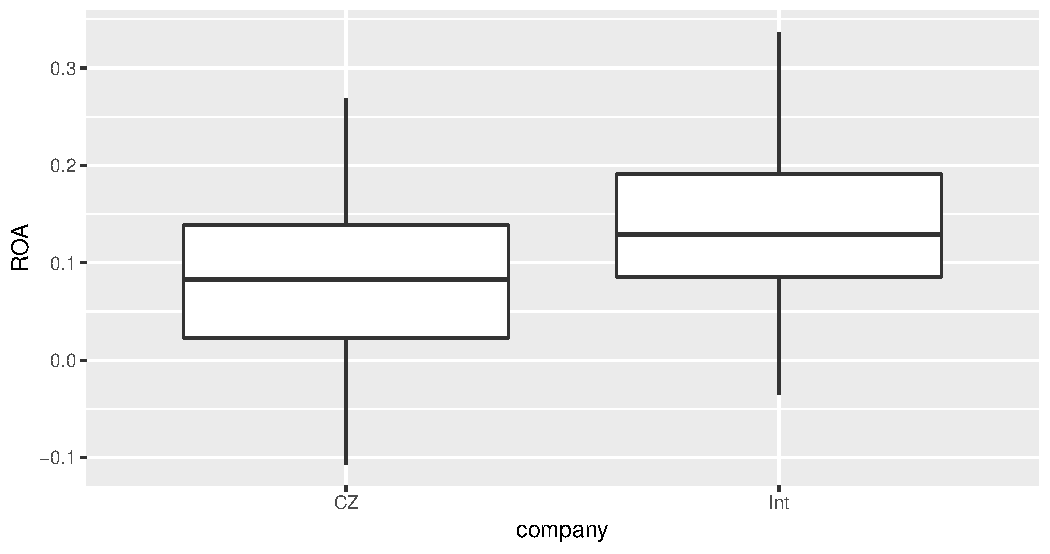
\includegraphics[width=1\textwidth]{figure/unnamed-chunk-20-1} 

}



\end{knitrout}

\end{frame}

%-----------

\begin{frame}[fragile]
\frametitle{Welch t-test: $\mu$ of first group is \textbf{less} than second}
\begin{knitrout}\footnotesize
\definecolor{shadecolor}{rgb}{0.969, 0.969, 0.969}\color{fgcolor}\begin{kframe}
\begin{alltt}
\hlkwd{t.test}\hlstd{(dataFin}\hlopt{$}\hlstd{ROA} \hlopt{~} \hlstd{dataFin}\hlopt{$}\hlstd{company,} \hlkwc{alternative}\hlstd{=}\hlstr{"less"}\hlstd{)}
\end{alltt}
\begin{verbatim}
## 
## 	Welch Two Sample t-test
## 
## data:  dataFin$ROA by dataFin$company
## t = -2.2853, df = 57.308, p-value = 0.01301
## alternative hypothesis: true difference in means is less than 0
## 95 percent confidence interval:
##         -Inf -0.01373392
## sample estimates:
##  mean in group CZ mean in group Int 
##        0.08528962        0.13645247
\end{verbatim}
\end{kframe}
\end{knitrout}

\end{frame}

%-----------

\begin{frame}[fragile]
\frametitle{When we just explore, no expectation }
\begin{knitrout}\footnotesize
\definecolor{shadecolor}{rgb}{0.969, 0.969, 0.969}\color{fgcolor}\begin{kframe}
\begin{alltt}
\hlkwd{t.test}\hlstd{(dataFin}\hlopt{$}\hlstd{ROA} \hlopt{~} \hlstd{dataFin}\hlopt{$}\hlstd{company)}
\end{alltt}
\begin{verbatim}
## 
## 	Welch Two Sample t-test
## 
## data:  dataFin$ROA by dataFin$company
## t = -2.2853, df = 57.308, p-value = 0.02601
## alternative hypothesis: true difference in means is not equal to 0
## 95 percent confidence interval:
##  -0.095987460 -0.006338226
## sample estimates:
##  mean in group CZ mean in group Int 
##        0.08528962        0.13645247
\end{verbatim}
\end{kframe}
\end{knitrout}

\end{frame}

%-----------

\begin{frame}[fragile]
\frametitle{Welch t-test: $\mu$ of first group is \textbf{greater}}
\begin{knitrout}\footnotesize
\definecolor{shadecolor}{rgb}{0.969, 0.969, 0.969}\color{fgcolor}\begin{kframe}
\begin{alltt}
\hlkwd{t.test}\hlstd{(dataFin}\hlopt{$}\hlstd{ROA} \hlopt{~} \hlstd{dataFin}\hlopt{$}\hlstd{company,} \hlkwc{alternative}\hlstd{=}\hlstr{"greater"}\hlstd{)}
\end{alltt}
\begin{verbatim}
## 
## 	Welch Two Sample t-test
## 
## data:  dataFin$ROA by dataFin$company
## t = -2.2853, df = 57.308, p-value = 0.987
## alternative hypothesis: true difference in means is greater than 0
## 95 percent confidence interval:
##  -0.08859177         Inf
## sample estimates:
##  mean in group CZ mean in group Int 
##        0.08528962        0.13645247
\end{verbatim}
\end{kframe}
\end{knitrout}

\end{frame}

\section{Regression Analysis}

%-----------

\begin{frame}\Huge\centering
Regression Analysis
\end{frame}

%-----------

\begin{frame}[fragile]\tiny

\begin{knitrout}
\definecolor{shadecolor}{rgb}{0.969, 0.969, 0.969}\color{fgcolor}\begin{kframe}
\begin{alltt}
\hlkwd{library}\hlstd{(ggplot2)}
\hlkwd{ggplot}\hlstd{(mtcars,} \hlkwd{aes}\hlstd{(}\hlkwc{x}\hlstd{=hp,} \hlkwc{y}\hlstd{=mpg) )} \hlopt{+}
  \hlkwd{geom_point}\hlstd{(}\hlkwc{size}\hlstd{=}\hlnum{2}\hlstd{,} \hlkwc{shape}\hlstd{=}\hlnum{21}\hlstd{,} \hlkwc{fill}\hlstd{=}\hlstr{"grey"}\hlstd{)} \hlopt{+}
  \hlkwd{geom_smooth}\hlstd{(}\hlkwc{method}\hlstd{=}\hlstr{"lm"}\hlstd{,} \hlkwc{se}\hlstd{=}\hlnum{FALSE}\hlstd{,} \hlkwc{color}\hlstd{=}\hlstr{"black"}\hlstd{)}
\end{alltt}
\end{kframe}

{\centering 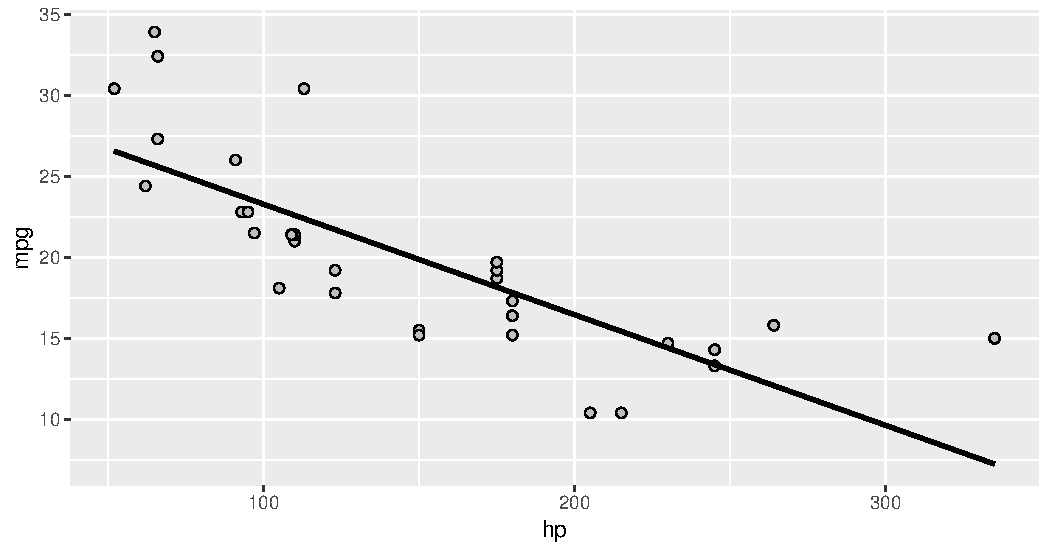
\includegraphics[width=1\textwidth]{figure/unnamed-chunk-24-1} 

}



\end{knitrout}

\end{frame}

%-----------

\begin{frame}[fragile]\large
\frametitle{Purpose of Regression Analysis}

The main purpose is to create a model of \textcolor{blue}{conditional} \textcolor{red}{expectation} of the \textcolor{orange}{dependent variable}. 

\begin{equation}
 \textcolor{red}{E}[\textcolor{orange}{y}\textcolor{blue}{\vert x}] \rightarrow y = f(x;\textcolor{magenta}{b}) 
\end{equation}

$f(\cdot)$ is a convenient function parametrised by parameters in vector $\textcolor{magenta}{b}$.

\begin{equation}
 y = \textcolor{magenta}{b_0} + \textcolor{magenta}{b_1}x_1 \nonumber
\end{equation}

\end{frame}

%-----------

\begin{frame}[fragile]
\frametitle{\textcolor{red}{E}[\textcolor{orange}{y}\textcolor{blue}{$\vert$x}]}

\begin{knitrout}
\definecolor{shadecolor}{rgb}{0.969, 0.969, 0.969}\color{fgcolor}

{\centering 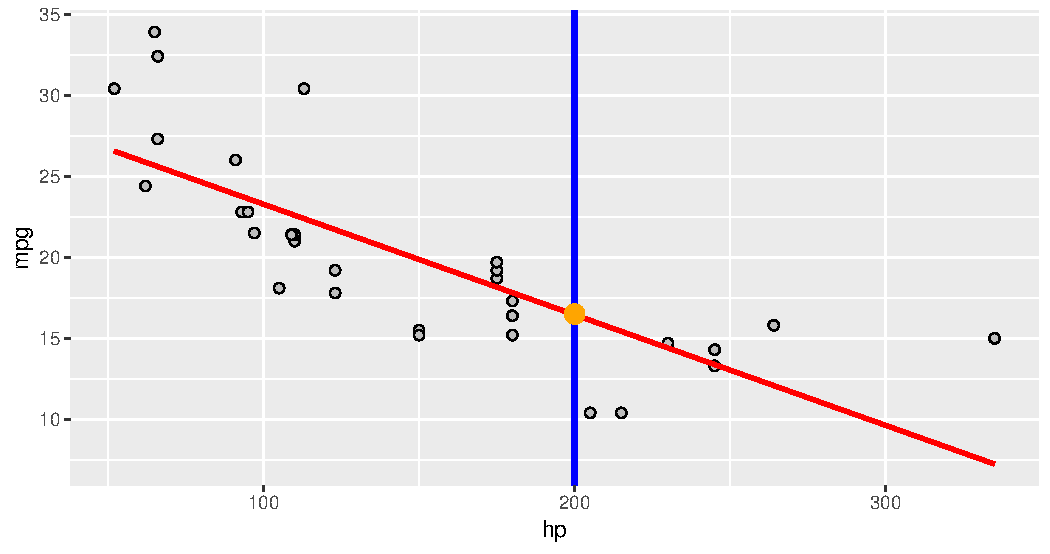
\includegraphics[width=1\textwidth]{figure/unnamed-chunk-25-1} 

}



\end{knitrout}

\onslide<2-> Unit increase of x leads to change in y by $b_1$... is usually wrong interpretation. The most important is the data design.

\end{frame}

%-----------

\begin{frame}
\frametitle{Linearity in Parameters}
\begin{Large}

 \begin{itemize}
	\item relation between $\beta$ is additive
	\item $\beta$ is not in a \emph{functional} form
 \end{itemize}
\begin{align}
y &= \beta_0 + \beta_1x_1 + \beta_2x_2 + \epsilon \\[0.4cm]
y &= \beta_0 + \beta_1\beta_2x_1 + \beta_3x_2 + \epsilon\\[0.4cm]
y &= \beta_0 + \beta_1^{\beta_2x_1} + \epsilon\\[0.4cm]
y &= \beta_0 + \sqrt{\beta_1}x_1 + \beta_2x_2 + \epsilon
\end{align}
\end{Large}
\end{frame}

%-----------

\begin{frame}\large
\frametitle{Linear model in parameters II}
\begin{equation}
y = \beta_0 + \beta_1x + \beta_2x^2 + \epsilon
\end{equation}

\begin{figure}
 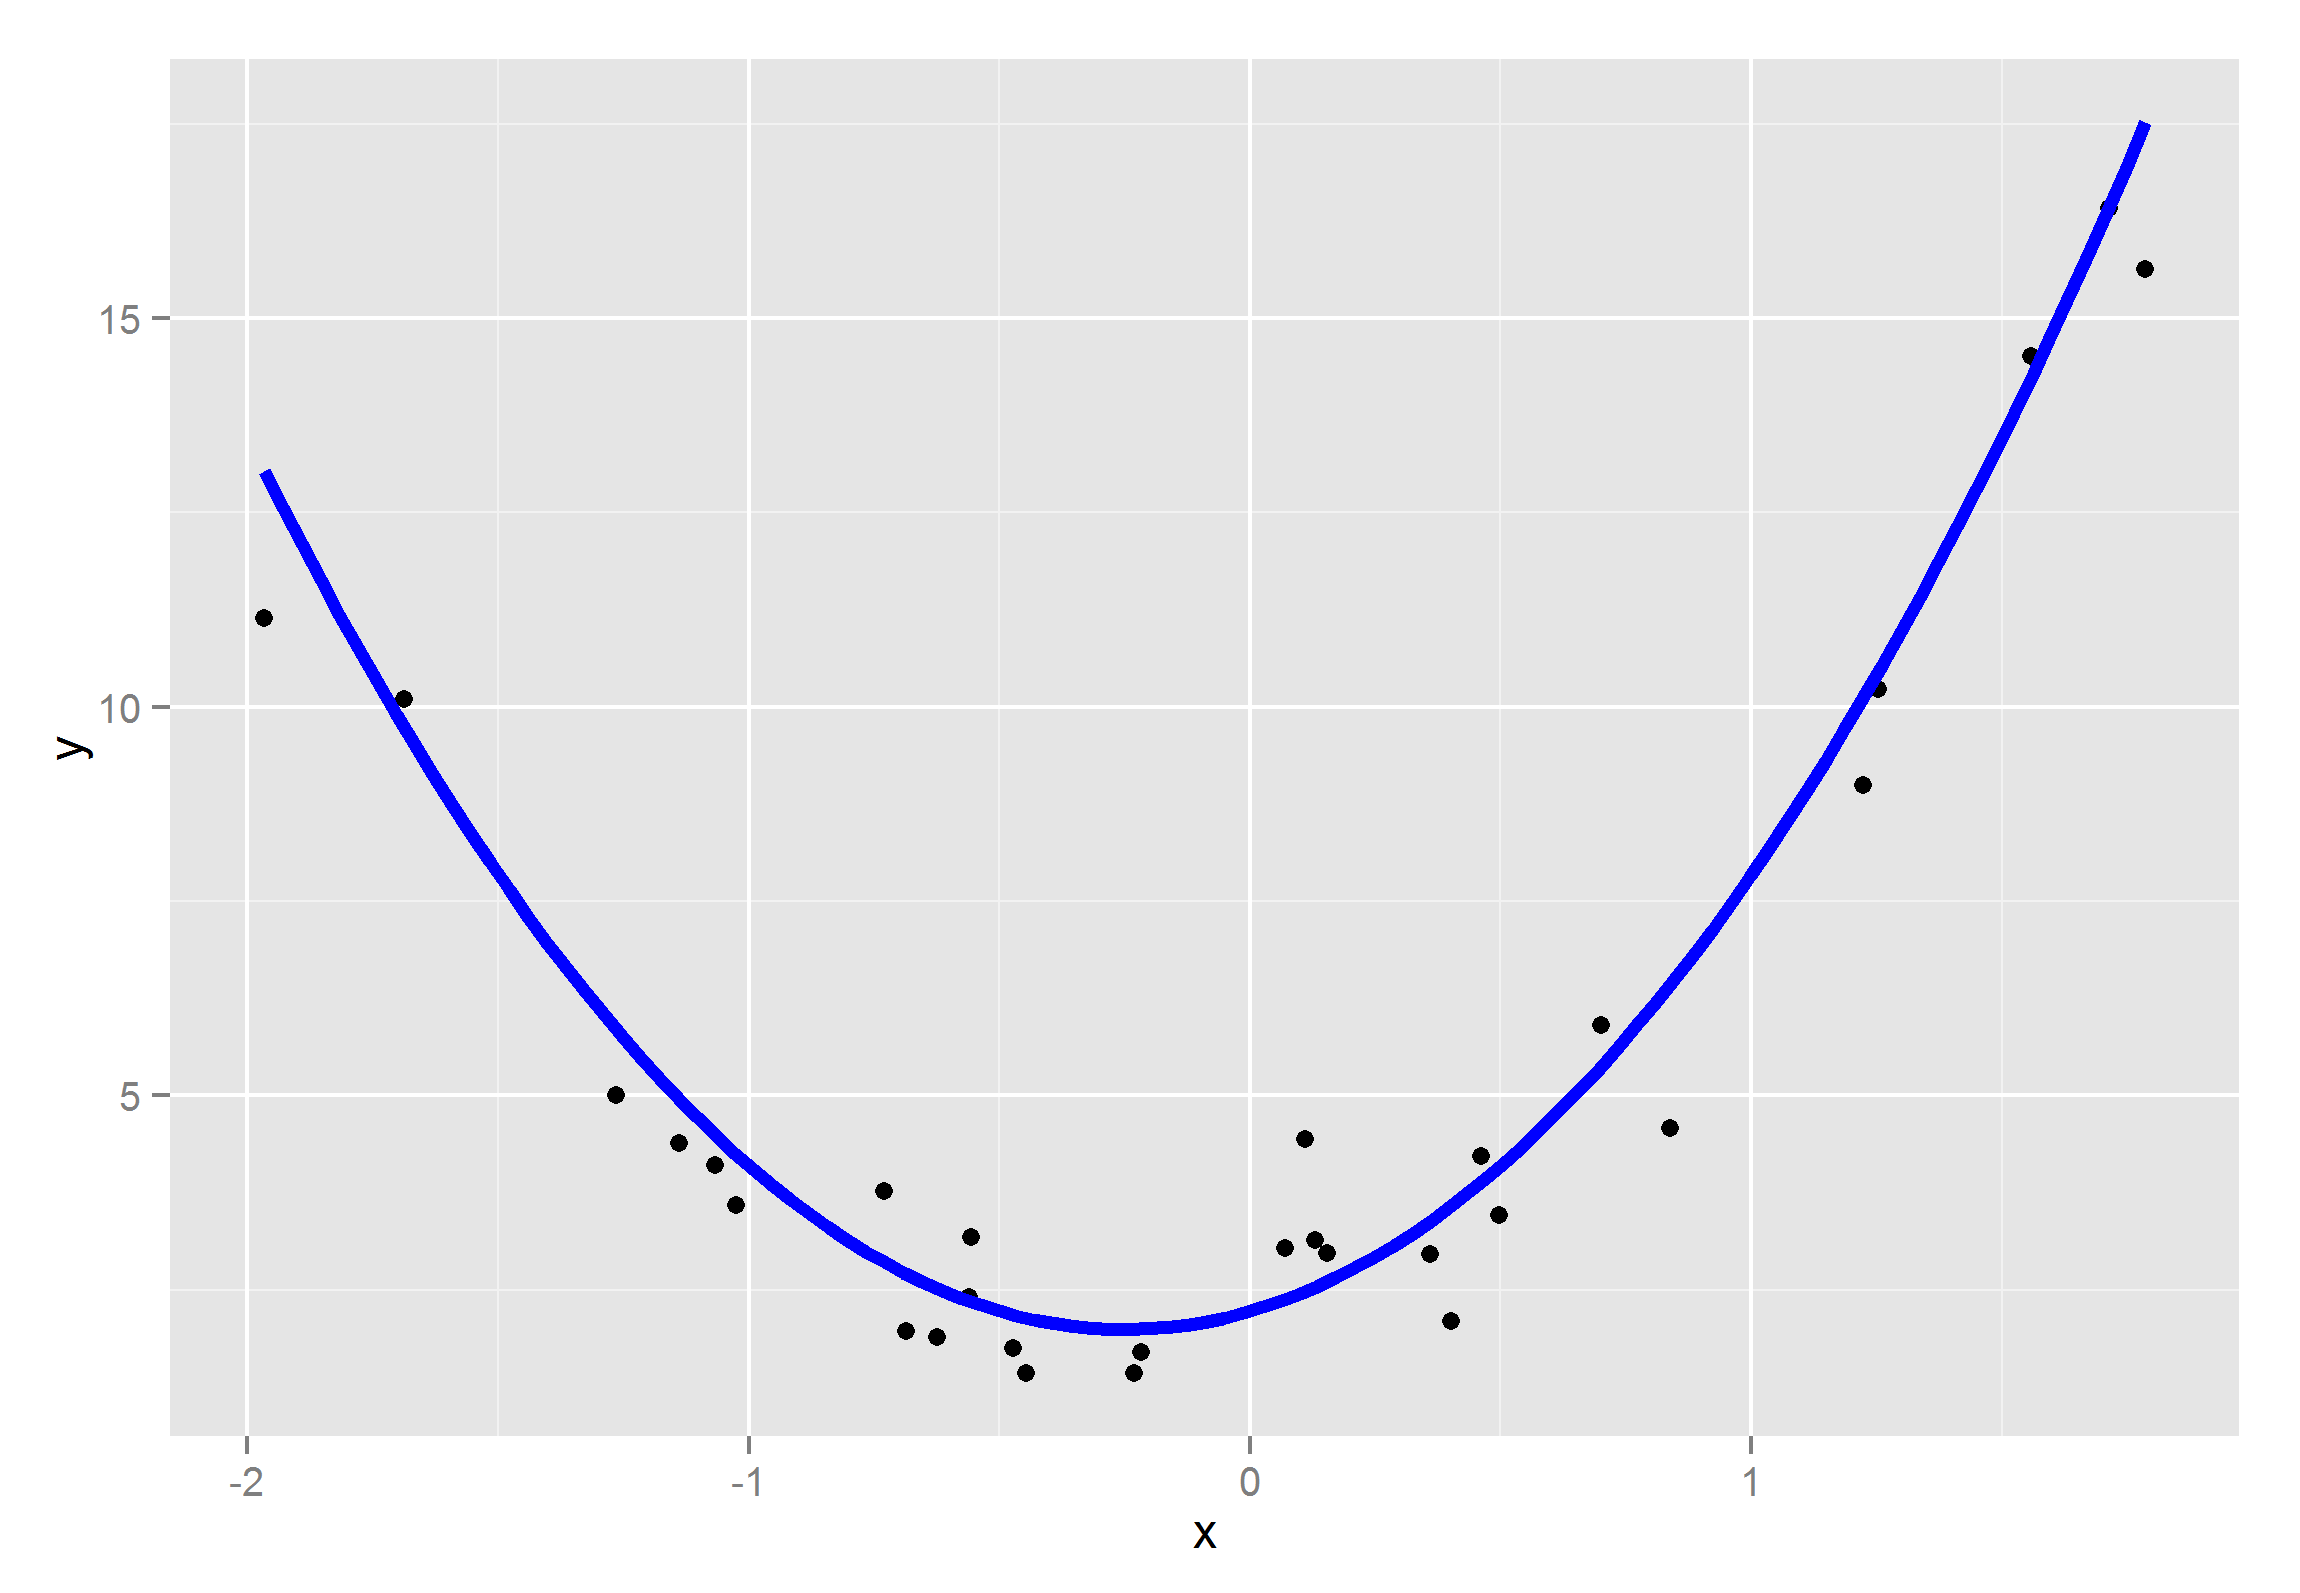
\includegraphics[width=0.7\paperwidth]{./Images/quadratic}
\end{figure}
\end{frame}

%-----------

\begin{frame}[fragile]\large
\frametitle{Linear Model}


If the model is linear in parameters, OLS method can be used to estimate parameters. In this case function \texttt{lm()} can be used:

\begin{knitrout}
\definecolor{shadecolor}{rgb}{0.969, 0.969, 0.969}\color{fgcolor}\begin{kframe}
\begin{alltt}
\hlstd{fit1} \hlkwb{<-} \hlkwd{lm}\hlstd{(mpg} \hlopt{~} \hlstd{hp,} \hlkwc{data}\hlstd{=mtcars)}
\end{alltt}
\end{kframe}
\end{knitrout}
Intercept ($b_0$) is added automatically. \onslide<2-> Consider model with intercept value only:

\begin{knitrout}
\definecolor{shadecolor}{rgb}{0.969, 0.969, 0.969}\color{fgcolor}\begin{kframe}
\begin{alltt}
\hlstd{fit0} \hlkwb{<-} \hlkwd{lm}\hlstd{(mpg} \hlopt{~} \hlnum{1}\hlstd{,} \hlkwc{data}\hlstd{=mtcars)}
\end{alltt}
\end{kframe}
\end{knitrout}

\end{frame}

%-----------

\begin{frame}[fragile]\footnotesize

\begin{knitrout}
\definecolor{shadecolor}{rgb}{0.969, 0.969, 0.969}\color{fgcolor}\begin{kframe}
\begin{alltt}
\hlkwd{summary}\hlstd{(fit0)}
\end{alltt}
\begin{verbatim}
## 
## Call:
## lm(formula = mpg ~ 1, data = mtcars)
## 
## Residuals:
##     Min      1Q  Median      3Q     Max 
## -9.6906 -4.6656 -0.8906  2.7094 13.8094 
## 
## Coefficients:
##             Estimate Std. Error t value Pr(>|t|)    
## (Intercept)   20.091      1.065   18.86   <2e-16 ***
## ---
## Signif. codes:  0 '***' 0.001 '**' 0.01 '*' 0.05 '.' 0.1 ' ' 1
## 
## Residual standard error: 6.027 on 31 degrees of freedom
\end{verbatim}
\end{kframe}
\end{knitrout}
\onslide<2->
\begin{knitrout}
\definecolor{shadecolor}{rgb}{0.969, 0.969, 0.969}\color{fgcolor}\begin{kframe}
\begin{alltt}
\hlkwd{mean}\hlstd{(mtcars}\hlopt{$}\hlstd{mpg)}
\end{alltt}
\begin{verbatim}
## [1] 20.09062
\end{verbatim}
\end{kframe}
\end{knitrout}

\end{frame}

%-----------

\begin{frame}[fragile]\footnotesize

\begin{knitrout}
\definecolor{shadecolor}{rgb}{0.969, 0.969, 0.969}\color{fgcolor}\begin{kframe}
\begin{alltt}
\hlkwd{summary}\hlstd{(fit1)}
\end{alltt}
\begin{verbatim}
## 
## Call:
## lm(formula = mpg ~ hp, data = mtcars)
## 
## Residuals:
##     Min      1Q  Median      3Q     Max 
## -5.7121 -2.1122 -0.8854  1.5819  8.2360 
## 
## Coefficients:
##             Estimate Std. Error t value Pr(>|t|)    
## (Intercept) 30.09886    1.63392  18.421  < 2e-16 ***
## hp          -0.06823    0.01012  -6.742 1.79e-07 ***
## ---
## Signif. codes:  0 '***' 0.001 '**' 0.01 '*' 0.05 '.' 0.1 ' ' 1
## 
## Residual standard error: 3.863 on 30 degrees of freedom
## Multiple R-squared:  0.6024,	Adjusted R-squared:  0.5892 
## F-statistic: 45.46 on 1 and 30 DF,  p-value: 1.788e-07
\end{verbatim}
\end{kframe}
\end{knitrout}

\end{frame}

%-----------

\begin{frame}[fragile]
\frametitle{Polynomial Regression}
There are two ways how to create polynomial (or log,...) regressions:
\begin{enumerate}
 \item Updating data before \texttt{lm}
 
\begin{knitrout}\footnotesize
\definecolor{shadecolor}{rgb}{0.969, 0.969, 0.969}\color{fgcolor}\begin{kframe}
\begin{alltt}
\hlstd{carsQuad} \hlkwb{<-} \hlstd{mtcars} \hlopt \hlkwd{select}\hlstd{(mpg, hp)} \hlopt
  \hlkwd{mutate}\hlstd{(}\hlkwc{hp2} \hlstd{= hp}\hlopt{^}\hlnum{2}\hlstd{)}

\hlkwd{lm}\hlstd{(mpg} \hlopt{~} \hlstd{hp} \hlopt{+} \hlstd{hp2,} \hlkwc{data}\hlstd{=carsQuad)} \hlopt \hlkwd{coef}\hlstd{()}
\end{alltt}
\begin{verbatim}
##   (Intercept)            hp           hp2 
## 40.4091172029 -0.2133082599  0.0004208156
\end{verbatim}
\end{kframe}
\end{knitrout}

\onslide<2-> \item Inside of \texttt{lm}
 
\begin{knitrout}\footnotesize
\definecolor{shadecolor}{rgb}{0.969, 0.969, 0.969}\color{fgcolor}\begin{kframe}
\begin{alltt}
\hlkwd{lm}\hlstd{(mpg} \hlopt{~} \hlstd{hp} \hlopt{+} \hlkwd{I}\hlstd{(hp}\hlopt{^}\hlnum{2}\hlstd{),} \hlkwc{data}\hlstd{=mtcars)} \hlopt \hlkwd{coef}\hlstd{()}
\end{alltt}
\begin{verbatim}
##   (Intercept)            hp       I(hp^2) 
## 40.4091172029 -0.2133082599  0.0004208156
\end{verbatim}
\end{kframe}
\end{knitrout}
 
\end{enumerate}



\end{frame}

%-----------

\begin{frame}\large
\frametitle{Coding of Variables}

$x=1$ means that highest achieved education level of a subject is a university degree. $x=0$ indicates non-university degree.
%
\begin{equation}
 \text{wage} = 20\,000 + 5\,000x \nonumber
\end{equation}
%
What if $x=1$ would mean non-university degree? \\[.4cm]

\onslide<2-> Redefine the model to have the same economic meaning.
\end{frame}

%-----------

\begin{frame}
\frametitle{Useful Packages}
\begin{knitrout}
\definecolor{shadecolor}{rgb}{0.969, 0.969, 0.969}\color{fgcolor}\begin{kframe}
\begin{alltt}
\hlkwd{library}\hlstd{(broom)}

\hlkwd{library}\hlstd{(car)}
\end{alltt}
\end{kframe}
\end{knitrout}

\end{frame}

%-----------

\begin{frame}[fragile]
\frametitle{R and Variable Coding}
Recall there is a variable \texttt{cyl} which takes only values  4, 6, 8. 


\begin{knitrout}\small
\definecolor{shadecolor}{rgb}{0.969, 0.969, 0.969}\color{fgcolor}\begin{kframe}
\begin{alltt}
\hlstd{fit2} \hlkwb{<-} \hlkwd{lm}\hlstd{(mpg} \hlopt{~} \hlstd{cyl, mtcars)}
\hlkwd{tidy}\hlstd{(fit2)}
\end{alltt}
\begin{verbatim}
## # A tibble: 2 x 5
##   term        estimate std.error statistic  p.value
##   <chr>          <dbl>     <dbl>     <dbl>    <dbl>
## 1 (Intercept)    37.9      2.07      18.3  8.37e-18
## 2 cyl            -2.88     0.322     -8.92 6.11e-10
\end{verbatim}
\end{kframe}
\end{knitrout}

What do you think about this model?
\end{frame}

%-----------

\begin{frame}[fragile]
\frametitle{}

\begin{knitrout}\small
\definecolor{shadecolor}{rgb}{0.969, 0.969, 0.969}\color{fgcolor}\begin{kframe}
\begin{alltt}
\hlstd{carData} \hlkwb{<-} \hlstd{mtcars} \hlopt
  \hlkwd{mutate}\hlstd{(}\hlkwc{cylinder} \hlstd{=} \hlkwd{factor}\hlstd{(cyl) )}
\end{alltt}
\end{kframe}
\end{knitrout}

\end{frame}

%-----------

\begin{frame}[fragile]
\frametitle{R and Variable Coding}
Recall there is a variable \texttt{cyl} which takes only values  4, 6, 8. 


\begin{knitrout}\small
\definecolor{shadecolor}{rgb}{0.969, 0.969, 0.969}\color{fgcolor}\begin{kframe}
\begin{alltt}
\hlstd{fit2.1} \hlkwb{<-} \hlkwd{lm}\hlstd{(mpg} \hlopt{~} \hlstd{cylinder, carData)}
\hlkwd{tidy}\hlstd{(fit2.1)}
\end{alltt}
\begin{verbatim}
## # A tibble: 3 x 5
##   term        estimate std.error statistic  p.value
##   <chr>          <dbl>     <dbl>     <dbl>    <dbl>
## 1 (Intercept)    26.7      0.972     27.4  2.69e-22
## 2 cylinder6      -6.92     1.56      -4.44 1.19e- 4
## 3 cylinder8     -11.6      1.30      -8.90 8.57e-10
\end{verbatim}
\end{kframe}
\end{knitrout}

This model is written as $y = b_0 + b_1x_1 + b_2x_2$ where $b_2=-11.6$ corresponds to the effect of 8 cylinders on \texttt{mpg}.
\end{frame}

%-----------

\begin{frame}[fragile]\small
\frametitle{Following Tests -- Wald test}

\begin{knitrout}
\definecolor{shadecolor}{rgb}{0.969, 0.969, 0.969}\color{fgcolor}\begin{kframe}
\begin{alltt}
\hlkwd{linearHypothesis}\hlstd{(fit2.1,} \hlstr{"cylinder6 = cylinder8"}\hlstd{,} \hlkwc{test}\hlstd{=}\hlstr{"F"}\hlstd{)}
\end{alltt}
\begin{verbatim}
## Linear hypothesis test
## 
## Hypothesis:
## cylinder6 - cylinder8 = 0
## 
## Model 1: restricted model
## Model 2: mpg ~ cylinder
## 
##   Res.Df    RSS Df Sum of Sq      F   Pr(>F)   
## 1     30 401.86                                
## 2     29 301.26  1    100.59 9.6835 0.004152 **
## ---
## Signif. codes:  0 '***' 0.001 '**' 0.01 '*' 0.05 '.' 0.1 ' ' 1
\end{verbatim}
\end{kframe}
\end{knitrout}

\end{frame}

%-----------

\begin{frame}[fragile]\small
\frametitle{Confidence Intervals}

\begin{knitrout}
\definecolor{shadecolor}{rgb}{0.969, 0.969, 0.969}\color{fgcolor}\begin{kframe}
\begin{alltt}
\hlstd{intervalsM2.1} \hlkwb{<-} \hlkwd{data.frame}\hlstd{(}\hlkwd{confint}\hlstd{(fit2.1))}
\hlstd{intervalsM2.1}
\end{alltt}
\begin{verbatim}
##                X2.5..   X97.5..
## (Intercept)  24.67608 28.651192
## cylinder6   -10.10796 -3.733599
## cylinder8   -14.21962 -8.907653
\end{verbatim}
\begin{alltt}
\hlkwd{colnames}\hlstd{(intervalsM2.1)} \hlkwb{<-} \hlkwd{c}\hlstd{(}\hlstr{"Low"}\hlstd{,} \hlstr{"Upp"}\hlstd{)}
\hlstd{intervalsM2.1}\hlopt{$}\hlstd{Estimate} \hlkwb{<-} \hlkwd{coef}\hlstd{(fit2.1)}
\hlstd{intervalsM2.1}
\end{alltt}
\begin{verbatim}
##                   Low       Upp   Estimate
## (Intercept)  24.67608 28.651192  26.663636
## cylinder6   -10.10796 -3.733599  -6.920779
## cylinder8   -14.21962 -8.907653 -11.563636
\end{verbatim}
\end{kframe}
\end{knitrout}

\end{frame}

%-----------

\begin{frame}[fragile]
\frametitle{}

\begin{knitrout}
\definecolor{shadecolor}{rgb}{0.969, 0.969, 0.969}\color{fgcolor}\begin{kframe}
\begin{alltt}
\hlkwd{ggplot}\hlstd{(intervalsM2.1,} \hlkwd{aes}\hlstd{(}
   \hlkwc{x}\hlstd{=}\hlkwd{rownames}\hlstd{(intervalsM2.1),} \hlkwc{y}\hlstd{=Estimate) )} \hlopt{+}
  \hlkwd{geom_point}\hlstd{()} \hlopt{+}
  \hlkwd{geom_errorbar}\hlstd{(}\hlkwd{aes}\hlstd{(}\hlkwc{ymin}\hlstd{=Low,} \hlkwc{ymax}\hlstd{=Upp),} \hlkwc{width}\hlstd{=}\hlnum{0.3}\hlstd{)}
\end{alltt}
\end{kframe}

{\centering 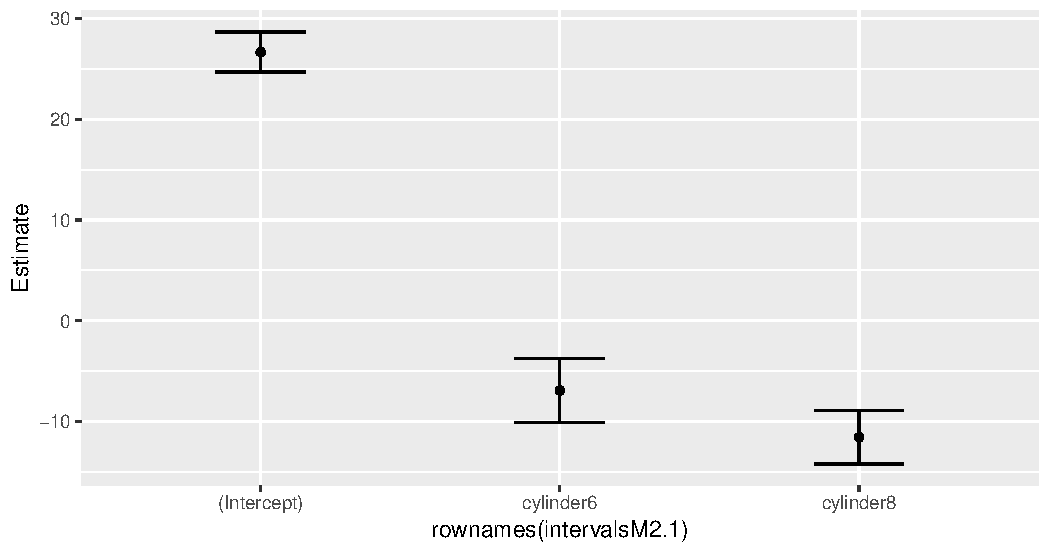
\includegraphics[width=1\textwidth]{figure/unnamed-chunk-39-1} 

}



\end{knitrout}

\end{frame}

\section{Time-Series Modelling}

\begin{frame}\Huge\centering
Time-Series 
\end{frame}

%-----------

\begin{frame}[fragile]
\frametitle{Useful Packages}
\begin{knitrout}
\definecolor{shadecolor}{rgb}{0.969, 0.969, 0.969}\color{fgcolor}\begin{kframe}
\begin{alltt}
\hlkwd{library}\hlstd{(forecast)} \hlcom{# Smoothing and many many more}

\hlkwd{library}\hlstd{(vars)} \hlcom{# Vector Autoregressive Models}

\hlkwd{library}\hlstd{(urca)} \hlcom{# unit-root and cointegration tests}

\hlkwd{library}\hlstd{(xts)} \hlcom{# Time-series objects}

\hlkwd{library}\hlstd{(lubridate)} \hlcom{# works with Date type}
\end{alltt}
\end{kframe}
\end{knitrout}

\textcolor{red}{Revolution in progress!} \texttt{library(tstibble)}, new version of \texttt{forecast} called \texttt{fable}.
\end{frame}

%-----------

\begin{frame}\large
\frametitle{Time Series}

\begin{itemize}
 \item Very different methodological approach (stationarity)
 \item Seasonality
 \item Time series is a set of autocorrelated values (unlike cross-sectional)
\end{itemize}

\textcolor{red}{\textsc{NEVER}} use standard Pearson Correlation test to analyse time-series!


\end{frame}


%-----------

\begin{frame}[fragile]
\frametitle{R Demonstration of Spurious Correlation}
\begin{knitrout}
\definecolor{shadecolor}{rgb}{0.969, 0.969, 0.969}\color{fgcolor}

{\centering 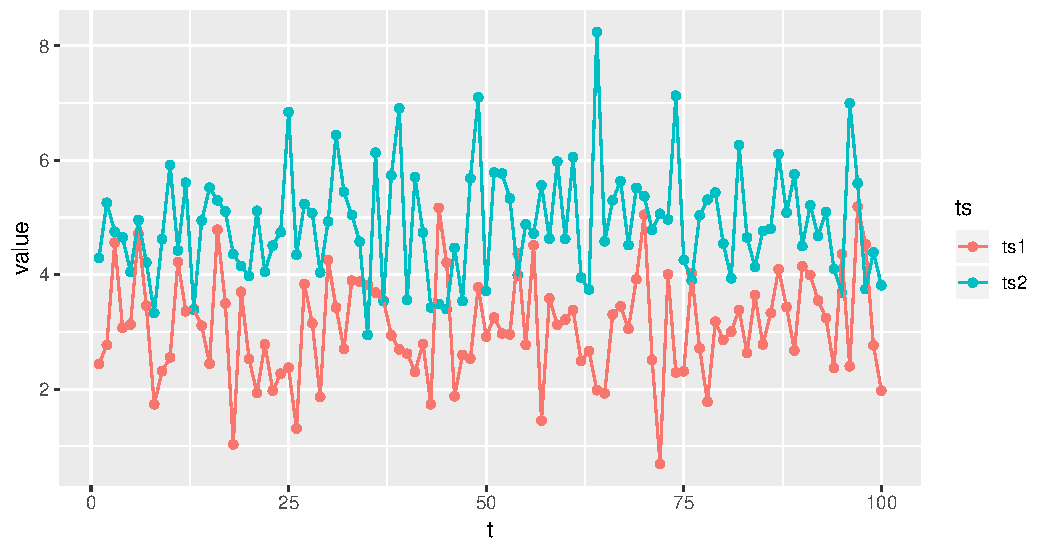
\includegraphics[width=1\textwidth]{figure/unnamed-chunk-41-1} 

}



\end{knitrout}
\begin{knitrout}
\definecolor{shadecolor}{rgb}{0.969, 0.969, 0.969}\color{fgcolor}\begin{kframe}
\begin{alltt}
\hlkwd{cor}\hlstd{(df}\hlopt{$}\hlstd{ts1, df}\hlopt{$}\hlstd{ts2)}
\end{alltt}
\begin{verbatim}
## [1] -0.04953215
\end{verbatim}
\end{kframe}
\end{knitrout}

\end{frame}

%-----------

\begin{frame}[fragile]\footnotesize
\begin{knitrout}
\definecolor{shadecolor}{rgb}{0.969, 0.969, 0.969}\color{fgcolor}\begin{kframe}
\begin{alltt}
\hlstd{df2} \hlkwb{<-} \hlstd{df} \hlopt \hlkwd{mutate}\hlstd{(}
 \hlkwc{ts1} \hlstd{= ts1} \hlopt{+} \hlnum{1.5} \hlopt{+} \hlnum{0.2}\hlopt{*}\hlkwd{seq}\hlstd{(}\hlnum{100}\hlstd{),}
 \hlkwc{ts2} \hlstd{= ts2} \hlopt{+} \hlnum{1.5} \hlopt{+} \hlnum{0.2}\hlopt{*}\hlkwd{seq}\hlstd{(}\hlnum{100}\hlstd{) )}
\end{alltt}
\end{kframe}
\end{knitrout}

\begin{knitrout}
\definecolor{shadecolor}{rgb}{0.969, 0.969, 0.969}\color{fgcolor}

{\centering 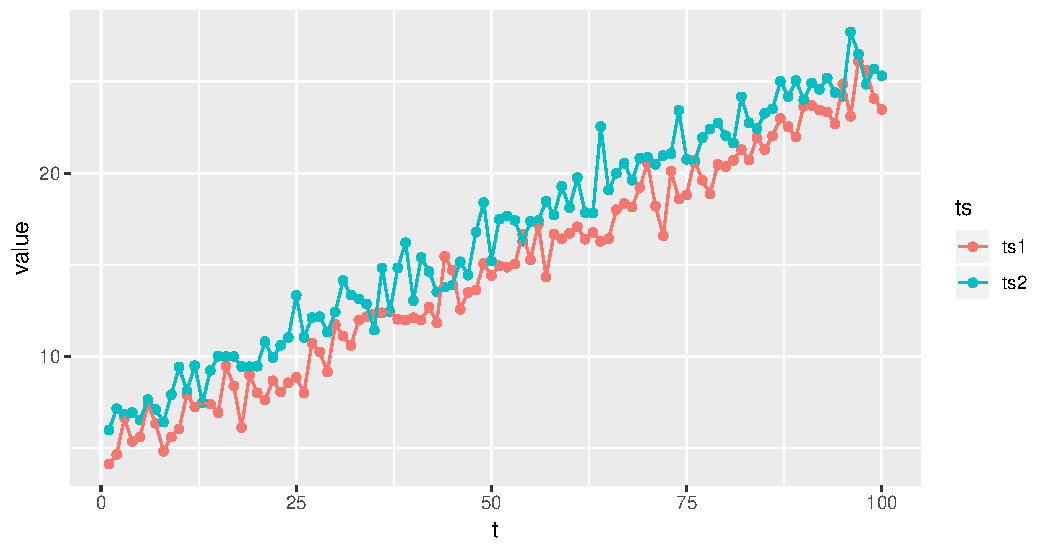
\includegraphics[width=1\textwidth]{figure/unnamed-chunk-44-1} 

}



\end{knitrout}
\onslide<2->
\begin{knitrout}
\definecolor{shadecolor}{rgb}{0.969, 0.969, 0.969}\color{fgcolor}\begin{kframe}
\begin{alltt}
\hlkwd{cor}\hlstd{(df2}\hlopt{$}\hlstd{ts1, df2}\hlopt{$}\hlstd{ts2)}
\end{alltt}
\begin{verbatim}
## [1] 0.9738829
\end{verbatim}
\end{kframe}
\end{knitrout}

\end{frame}

%-----------

\begin{frame}\frametitle{Spurious Correlation}
 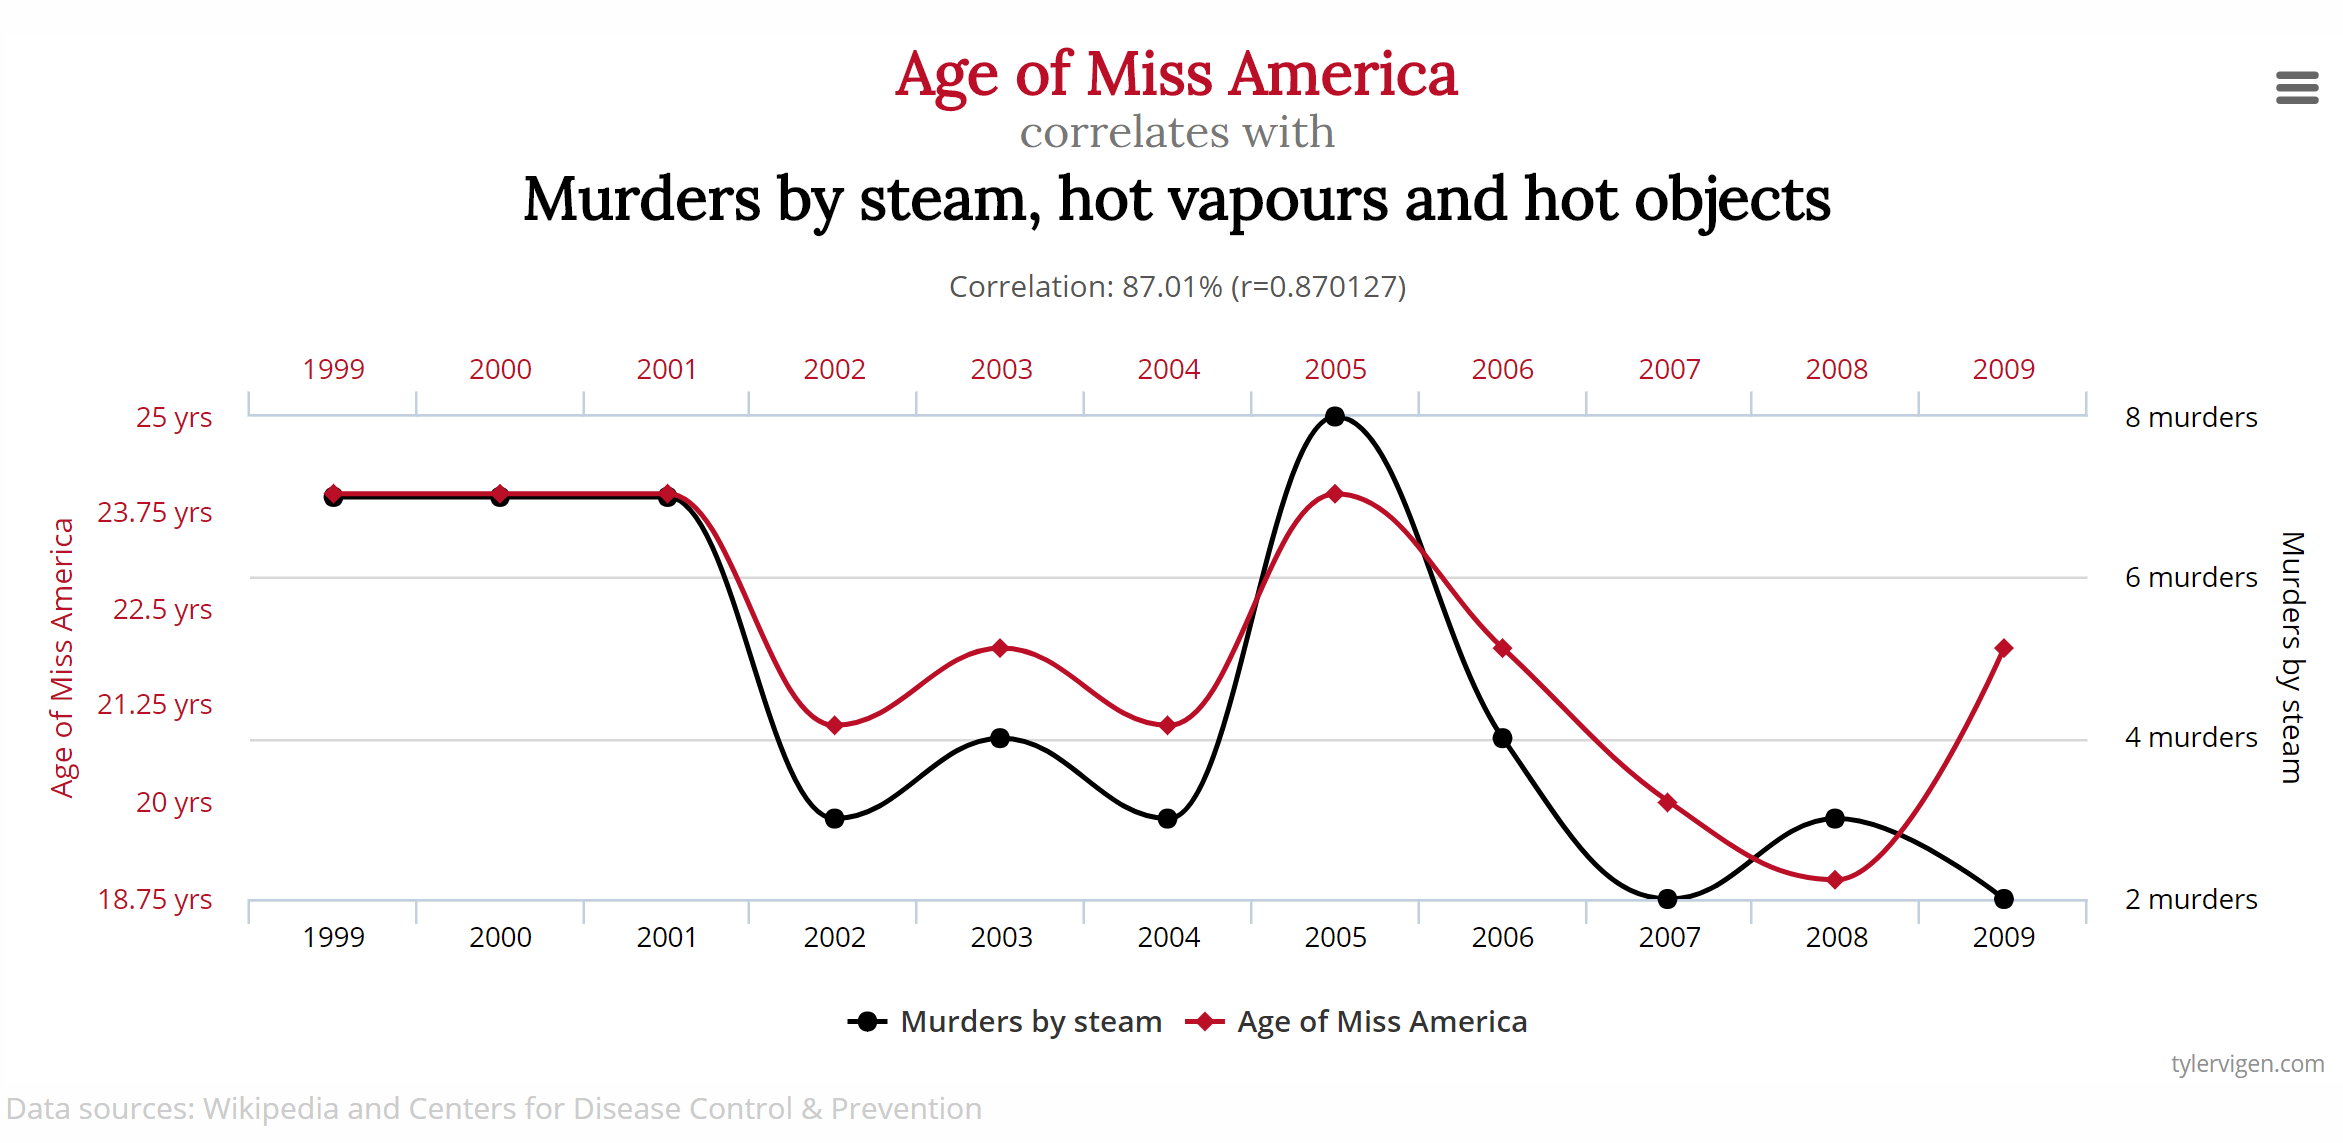
\includegraphics[height=0.8\paperheight,width=0.8\paperwidth]{./Images/spurious}
\end{frame}

%-----------

\begin{frame}\large
\frametitle{Stationarity}

Assumption that the time series has a constant mean and variance (weak form of definition).

This needs to be tested:

\begin{itemize}
 \item stochastic stationarity (SS) - ADF test, PP test,...
 \item deterministic stationarity (DS) - KPSS test
\end{itemize}

It is important to distinguish between two types. SS time series can be made stationary by differencing, DS time series by removing trend (e.g., by using OLS).


\end{frame}

%-----------

\begin{frame}[fragile]\footnotesize

\begin{knitrout}
\definecolor{shadecolor}{rgb}{0.969, 0.969, 0.969}\color{fgcolor}\begin{kframe}
\begin{alltt}
\hlkwd{library}\hlstd{(tseries)}
\hlkwd{adf.test}\hlstd{(df}\hlopt{$}\hlstd{ts1)}
\end{alltt}


{\ttfamily\noindent\color{warningcolor}{\#\# Warning in adf.test(df\$ts1): p-value smaller than printed p-value}}\begin{verbatim}
## 
## 	Augmented Dickey-Fuller Test
## 
## data:  df$ts1
## Dickey-Fuller = -4.3961, Lag order = 4, p-value = 0.01
## alternative hypothesis: stationary
\end{verbatim}
\end{kframe}
\end{knitrout}

\end{frame}

%-----------

\begin{frame}[fragile]\footnotesize

\begin{knitrout}
\definecolor{shadecolor}{rgb}{0.969, 0.969, 0.969}\color{fgcolor}\begin{kframe}
\begin{alltt}
\hlkwd{adf.test}\hlstd{(df2}\hlopt{$}\hlstd{ts1)}
\end{alltt}


{\ttfamily\noindent\color{warningcolor}{\#\# Warning in adf.test(df2\$ts1): p-value smaller than printed p-value}}\begin{verbatim}
## 
## 	Augmented Dickey-Fuller Test
## 
## data:  df2$ts1
## Dickey-Fuller = -4.3961, Lag order = 4, p-value = 0.01
## alternative hypothesis: stationary
\end{verbatim}
\end{kframe}
\end{knitrout}

\end{frame}

%-----------


\begin{frame}[fragile]\large
\frametitle{Kwiatkowski et al. test}
$H_0$: Time series is trend stationary:
\begin{knitrout}
\definecolor{shadecolor}{rgb}{0.969, 0.969, 0.969}\color{fgcolor}\begin{kframe}
\begin{alltt}
\hlkwd{kpss.test}\hlstd{(df}\hlopt{$}\hlstd{ts1)}\hlopt{$}\hlstd{p.value}
\end{alltt}
\begin{verbatim}
## [1] 0.1
\end{verbatim}
\begin{alltt}
\hlkwd{kpss.test}\hlstd{(df2}\hlopt{$}\hlstd{ts1)}\hlopt{$}\hlstd{p.value}
\end{alltt}
\begin{verbatim}
## [1] 0.01
\end{verbatim}
\end{kframe}
\end{knitrout}
If rejected, de-trending will help.

\end{frame}

%-----------

\begin{frame}\large
\frametitle{Other Useful Functions}

\begin{itemize}
 \item stl -- time-series decomposition
 \item ccf -- cross-correlation
 \item Arima 
 \item var
\end{itemize} 
 
\end{frame}

%-----------

\begin{frame}\centering\Large
Thank you! \bigskip 

homolka@utb.cz\bigskip 

\href{https://github.com/luboRprojects/tidyWorkshop}{
\includegraphics[width=0.1\textwidth,height=0.1\textheight,keepaspectratio]{./Images/github}}


%\href{https://stackoverflow.com/users/7357438/lstat?tab=profile}{\includegraphics[width=0.3\textwidth,height=0.3\textheight,keepaspectratio]{./Images/stackoverflow}}

\end{frame}

\end{document}
